\documentclass[9pt]{sigplanconf}

\newcommand{\DSU}{{\sc Jvolve}}
\newcommand{\transformObject}{\texttt{jvolveObject}}
\newcommand{\transformClass}{\texttt{jvolveClass}}
\newcommand{\VMClass}{\texttt{RVMClass}}
\newcommand{\TIB}{\texttt{TIB}}
\newcommand{\JTOC}{\texttt{JTOC}}
\newcommand{\JikesRVM}{Jikes RVM}
\newcommand{\JRVMVersion}{Jikes RVM (SVN r15532)}

% This is for adjusting spacing in tables
% Taken from
% https://www.msu.edu/~harris41/latex_tablespacing.html
\newcommand\T{\rule{0pt}{2.0ex}}
\newcommand\B{\rule[-1.2ex]{0pt}{0pt}}

\usepackage{times}
\usepackage{rotating}
\usepackage{subfigure}
\usepackage{acronym}
\usepackage{multirow}
\usepackage{graphics}
\usepackage{float}
\usepackage{setspace}
\usepackage{url}
\usepackage[usenames]{color}
\usepackage[override]{cmtt}
% \usepackage{hyperref}

% \newcommand\maybecolor[1]{\color{#1}}
% \newcommand\mwh[1]{{\maybecolor{green}\textbf{Mike says:} #1}}
% \newcommand\ksm[1]{{\maybecolor{blue}\textbf{Kathryn says:} #1}}
% \newcommand\suriya[1]{{\maybecolor{blue}\textbf{Suriya says:} #1}}
% \newcommand\todo[1]{{\maybecolor{red} #1}}
% \newcommand\proofread[1]{{\maybecolor{red} #1}}
% \newcommand\mwh[1]{}
% \newcommand\ksm[1]{}
% \newcommand\suriya[1]{}
% \newcommand\todo[1]{}

\begin{document}

\conferenceinfo{PLDI'09,} {June 15--20, 2009, Dublin, Ireland.}
\CopyrightYear{2009}
\copyrightdata{978-1-60558-392-1/09/06}

\title{Dynamic Software Updates: A VM-centric Approach}
\authorinfo{Suriya Subramanian}{The University of Texas at Austin}{suriya@cs.utexas.edu}
\authorinfo{Michael Hicks}{University of Maryland, College Park}{mwh@cs.umd.edu}
\authorinfo{Kathryn S. McKinley}{The University of Texas at Austin}{mckinley@cs.utexas.edu}
\maketitle

%%% TEXEXPAND: INCLUDED FILE MARKER ./abstract.tex
\subsection*{Abstract}
Software evolves to fix bugs and add features. Stopping and restarting
programs to apply changes is inconvenient and often costly.  Dynamic
software updating (DSU) addresses this problem by updating programs
while they execute, but existing DSU systems for managed languages do
not support many updates that occur in practice and are inefficient.
This paper presents the design and implementation of \DSU, a
DSU-enhanced Java VM.  Updated programs may add, delete, and replace fields
and methods anywhere within the class hierarchy.  \DSU{} implements
these updates by adding to and coordinating VM classloading,
just-in-time compilation, scheduling, return barriers, on-stack
replacement, and garbage collection.  \DSU{} is \emph{safe}: its use
of bytecode verification and VM thread synchronization ensures that an
% ISSUE: no bytecode verification in JikesRVM
update will always produce type-correct executions. \DSU{} is
\emph{flexible}: it can support 20 of 22 updates to three
open-source programs---Jetty web server, JavaEmailServer, and CrossFTP
server---based on actual releases occurring over 1 to 2 years.
%REFACTOR: though slight refactorings would allow the other updates.
\DSU{} is \emph{efficient}: performance experiments show that
\DSU{} incurs \emph{no overhead} during steady-state execution.  These
results demonstrate that this work is a significant step towards
practical support for 
dynamic updates in virtual machines for managed languages.

%%% Local Variables: 
%%% mode: latex
%%% TeX-master: "pldi64"
%%% End: 
%%% TEXEXPAND: END FILE ./abstract.tex

\category{D.3.4}{Programming Languages}{Processors}[Run-time environments]
\terms Languages, Experimentation, Reliability
\keywords dynamic software updating, virtual machine technology, garbage collection 

%%% TEXEXPAND: INCLUDED FILE MARKER ./intro.tex
% $Id: intro.tex 9934 2009-03-31 09:49:43Z mwh657 $

\section{Introduction}

Software is imperfect.  To fix bugs and adapt software to user
demands, developers must modify deployed systems.  However, halting a
software system to apply updates creates new problems: safety concerns
for mission-critical and transportation systems; substantial revenue
losses for businesses~\cite{gartner98downtime,roc1}; maintenance
costs~\cite{zorn05}; and at the least, inconvenience for users. These
problems may translate into serious security risks if patches are not
applied promptly~\cite{altekar05opus,ksplice}.  

Dynamic software updating (DSU) is a general-purpose mechanism that
solves these problems by updating programs while they run without a
special software architecture or redundant
hardware~\cite{kspliceslashdot08}. A practical DSU system must be safe,
flexible, and efficient.  \emph{Safe} updates insure the program is as
correct as deploying it from scratch.  The update model would ideally
be \emph{flexible} enough to support all software changes, but DSU is
still useful if the system supports most software updates.  Since
updates should be rare events, an \emph{efficient} DSU system would
ideally impose no 
runtime overhead during steady-state program execution.

Researchers have made significant strides toward making DSU practical
for systems written in C or C++, supporting server feature
upgrades~\cite{neamtiu06dsu,chen:icse07,upstare}, security
patches~\cite{altekar05opus}, and operating systems
upgrades~\cite{K42reconfig,k42usenix,baumann07reboots,dynamos_eurosys_07,chen06vee,ksplice}.
Enterprise systems and embedded systems---including safety-critical
applications---are increasingly written in managed languages, such as
Java, Ruby, and C\#.  Unfortunately, work on DSU for managed languages
lags behind work for C and C++.  For example, while the HotSpot
JVM~\cite{JVMhotswap} and some .NET languages~\cite{VSEnC} support
on-the-fly method body updates, this support is too inflexible for all
but the simplest updates---limiting changes to method bodies would
support less than half of the updates
to our three Java benchmark programs.  Academic
approaches~\cite{ritzau00dynamic,Mala00a,orso:java,bierman08upgradej} offer more
flexibility, but have not been proven on realistic applications.
Furthermore, they employ method
and object indirection to make applications DSU capable, imposing substantial space
and time overheads on steady-state execution.

This paper presents the design of \DSU, a DSU system for Java, which
we implement in \JikesRVM, a Java Virtual Machine. \DSU's combination
of flexibility, safety, and efficiency is a clear advance over prior
approaches.  The 
paper's key contribution is to show how to extend and integrate
existing VM services to support DSU that is flexible enough to support
a large class of updates, guarantees type-safety, and imposes no space
or time overheads on steady-state execution.
% \DSU{} is built on 
% \JikesRVM, a Java research virtual machine.
% \suriya{Say that Jvolve is built on top of JikesRVM. Reviewer 4 wanted us
% to say this earlier}

\DSU{} DSU supports many common updates. Users can add, delete, and
change existing classes.  Changes may add or remove fields and methods,
replace existing ones, and change type signatures.  Changes may occur
at any level of the class hierarchy.  To initialize new fields and
update existing ones, \DSU{} applies \emph{class} and \emph{object
  transformer} functions, the former for static fields and the latter
for object instance fields.  The system automatically generates
default transformers, which initialize new and changed fields to
default values and retain values of unchanged fields.  If needed,
programmers may customize the default transformers.

%MWH: Suriya asserted that we don't rely on bytecode verification.
%Are you saying that we don't actually verify the classes we load in?
%If we do, we get assurances of type safety, right?
% bytecode verification is a specific term to describe a technology that
% JVMs use to assure the safety/correctness of the loaded bytecode.
% JikesRVM does not have a bytecode verifier.
\DSU{} relies on bytecode verification to statically type-check
% ISSUE: no bytecode verification in JikesRVM
updated classes.  To avoid type errors due to the timing of an
update~\cite{StoyleHBSN06,neamtiu06dsu,k42usenix}, \DSU{} stops the executing
threads at a \emph{DSU safe point} and then applies the update. DSU
safe points are a subset of VM \emph{safe points}, where it is safe to perform garbage collection (GC) and thread scheduling.  DSU safe points further
restrict the methods that may be on each thread's stack, depending on
the update.  These methods include (1) updated methods,
(2) methods that refer to updated classes (since their machine code 
may contain hard-coded offsets that the update changes), and (3) user-specified methods
as needed for safety~\cite{Gupta94,neamtiu08context}.  \DSU{} installs return
barriers~\cite{return-barrier} on these methods to inform the run-time system when
a running method returns, to speed up reaching a safe point.  \DSU{}
also applies on-stack replacement (OSR) to recompile methods in the
second category even as they run, as long as they do not contain inlined
updated methods.  This approach does not guarantee \DSU{} will reach a DSU safe point, but in our
multithreaded benchmarks it does in nearly all cases. More sophisticated
thread scheduling support could attain greater
flexibility~\cite{neamtiu09stump}. 

\DSU{} makes use of the garbage collector and JIT compiler to
efficiently update the code and data associated with changed classes.
\DSU{} initiates a whole-heap GC to find existing object
instances of updated classes and initialize new versions using the
provided object transformers.  \DSU{} invalidates existing compiled 
code and installs new bytecode for all changed method implementations.
When the application resumes execution these methods
are JIT-compiled when they are next invoked.
The adaptive compilation system naturally optimizes updated methods
further if they execute frequently.

\DSU{} imposes no overhead during steady-state execution.  During an
update, it imposes overheads in 
classloading and garbage collection. After an update, the adaptive
compilation system will incrementally optimize the updated code in its
usual fashion.  Eventually, the code is fully optimized and running
with no additional overhead.  The zero overhead in steady-state
execution for a
VM-based approach is in contrast to DSU techniques for C and C++. These
approaches
must use a compiler or dynamic rewriter to insert levels of
indirection~\cite{neamtiu06dsu, orso:java} or
trampolines~\cite{chen06vee,chen:icse07,altekar05opus,ksplice}, which
add a constant overhead during normal execution.
% Garbage collection also
% provides substantial flexibility.  Rather than padding objects in case they
% become larger due to an update~\cite{neamtiu06dsu}, the collector
% copies changed objects, grows them only if necessary, and thus
% supports a richer set of updates.

We assessed \DSU{} by applying updates corresponding to
one to two years' worth of releases of three open-source
multithreaded applications: Jetty web server,
JavaEmailServer (an SMTP and POP server), and CrossFTP server.  We
found that \DSU{}
can successfully apply 20 of the 22 updates---the two updates it does
not support change a method within an infinite loop that is always on the
stack.
% REFACTOR: add sentence here about the Jetty refactoring, if we can get
% that to work.
Microbenchmark results show that the pause time due to an
update depends on the size of the heap and fraction of transformed
objects. 
% Compared to the highly-optimized copy operation the GC would
% normally use, our compilation of user-provided object transformers is
% significantly slower, which in the limit could incur a high cost.
% However, most updates transform only a small fraction of heap objects
% and this cost is incurred only during the update itself.
Experiments
with Jetty show that applications updated by \DSU{} enjoy the same
steady-state performance as if started from scratch.

In summary, this paper's main contributions are (1) techniques to extend and
integrate standard virtual machine services for managed languages to
support flexible, safe, and efficient dynamic software updating
services, (2) the design, implementation, and evaluation of \DSU, a
Java VM with support for dynamic software updating. \DSU{} is
distinguished from prior work in its realism, flexibility, technical
novelty, and high performance.  We believe our demonstration is a
significant step towards supporting flexible, efficient, and safe
updates in managed code virtual machines.
%% The remainder of the paper first
%% compares our approach carefully to related work, and then describes
%% our model of updates, our implementation, and experimental results.

%%% Local Variables: 
%%% mode: latex
%%% TeX-master: "pldi64"
%%% End: 
%%% TEXEXPAND: END FILE ./intro.tex
%%% TEXEXPAND: INCLUDED FILE MARKER ./model.tex


\begin{figure}[t]
\begin{center}
\scalebox{.67}{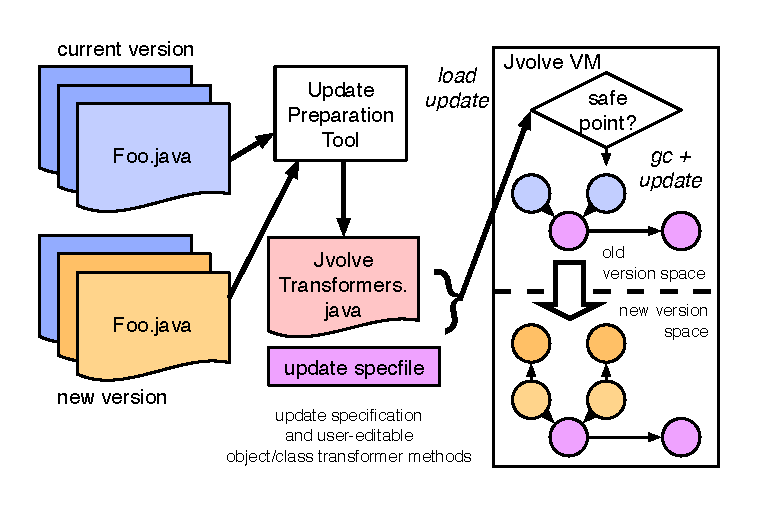
\includegraphics{images/system}}
\end{center}
\caption{Dynamic Software Updating with \DSU}
\label{fig:overview}
\end{figure}


%MWH: I don't think this section is particularly about a VM-centric
%   design.  I've reverted the text back to the way it was.  The next
%   section is about the VM.  We'd have to make more significant
%   changes here, not sure how, to somehow claim this is an overview
%   of VM-centric DSU.  The approach here, modulo the discussion of
%   garbage collection, could just as well apply to a system
%   implemented via rewriting.

% \section{A VM-centric DSU Design}

% This section begins by overviewing a VM-centric approach, our design
% choices, update model, and describes how the developer participates in
% the process. Section~\ref{sec:vm} describes each component in detail.

\section{Dynamic Updates in \DSU}

This section overviews \DSU's approach, what changes it permits, and
how the developer participates in the process.

\subsection{System Overview}
\label{sec:overview}

Figure~\ref{fig:overview} illustrates the dynamic update process.
Assume that the VM is executing the current version of the program,
whose code is depicted in the left top corner.  Meanwhile, developers
prepare a new version and fully test it using standard procedures.
A developer 
then invokes \DSU's \ac{UPT} on the old and
new versions. The \ac{UPT} generates an update specification, which identifies
new and updated classes, and a \texttt{JvolveTransformers.java} file
that contains default \emph{object}
and \emph{class transformer} methods.  

Transformer methods take an
object or class of the old version and 
initialize the corresponding object or class of the new version.  The default
transformers assign default values, such as zero and {\tt null}, to new
instance, reference, and static fields, and copy values for unchanged
fields.  Developers may customize the default transformers as
necessary.  We present an example update and transformer in
Section~\ref{subsec:transformers}. %, and briefly discuss how they are compiled.

The user signals the running VM to apply the update, and the VM loads
the new class files and transformers and schedules the update. The VM
scheduler signals an interrupt, which stops all threads at
VM safe points, where it is safe to perform thread scheduling and garbage collection.  \DSU{} then checks if the VM is % also
at a \emph{DSU safe point}. DSU safe points require that no thread's
activation stack contains a \emph{restricted} method.  Restricted
methods are of three categories: (1) methods changed by the update,
(2) methods whose bytecode is unchanged but whose compiled
representation may change, and (3) methods specified by the user. If
restricted methods are on stack, the VM installs return-barriers
for~(1) and~(3), and performs on-stack-replacement for~(2) to reach a
DSU safe point.  Section~\ref{sec:safe} describes this process in
detail.

Once all application threads have synchronized at DSU safe points, \DSU{}
applies the update. It first invalidates the compiled versions of all
changed methods.
These methods are
recompiled as needed---the adaptive JIT compiler will
generate code the next time the program invokes an invalidated method,
and may optimize it further, if the program executes it frequently.
%
The VM then invokes the
class transformers.  Finally, the VM initiates a full copying garbage collection. It
piggybacks on the garbage collector to detect all existing objects
whose classes change. It allocates objects that conform to the new type
declarations, and performs object transformations to populate the new
objects with valid state. %, as described above.  
At this point, the update is complete.

%%% TEXEXPAND: INCLUDED FILE MARKER ./running-example.tex
\begin{figure*}[t]
\begin{tabular}{c|c}
\begin{minipage}{3.12in}
\begin{small}
\begin{verbatim}
public class User {
  private final String username, domain, password;
  private String[] forwardAddresses;
  public User(...) {...}
  public String[] getForwardedAddresses() {...}
  public void setForwardedAddresses(String[] f) {...}
}
public class ConfigurationManager {
  private User loadUser(...) {
     ...
     User user = new User(...);
     String[] f = ...;
     user.setForwardedAddresses(f);
     return user;
  }
}
\end{verbatim}
\end{small}
\end{minipage} &
\begin{minipage}{3.5in}
\begin{small}
\begin{verbatim}
public class User {
  private final String username, domain, password;
  private EmailAddress[] forwardAddresses;
  public User(...) {...}
  public EmailAddress[] getForwardedAddresses() {...}
  public void setForwardedAddresses(EmailAddress[] f) {...}
}
public class ConfigurationManager {
  private User loadUser(...) {
     ...
     User user = new User(...);
     EmailAddress[] f = ...;
     user.setForwardedAddresses(f);
     return user;
  }
}
\end{verbatim}
\end{small}
\end{minipage} \\
(a) Version 1.3.1 &
(b) Version 1.3.2 \\
\end{tabular}
\caption{Example changes to JavaEmailServer \texttt{User} and
  \texttt{ConfigurationManager} classes}
\label{fig:email-example}
\end{figure*}

% vim:nospell
%%% TEXEXPAND: END FILE ./running-example.tex

\subsection{Programmer Update Model}
\label{sec:updates}

We have designed a flexible, yet simple update model that supports
updates that we believe are important in practice. 

Programmers may
change method bodies. Method body updates are the simplest and most
commonly supported
change~\cite{JVMhotswap, VSEnC, eaddy05enc, GilmoreKW97, orso:java,
  K42reconfig, HjalmtyssonG98},
because DSU systems can preserve type safety by simply invoking the new
method the next time the program executes the method.  However,
restricting updates to method bodies prevents many common
changes~\cite{neamtiu05evolution}.  Section~\ref{sec:experience} shows
% Suriya: changed shows to will show
%MWH: this should be present tense.  A document always shows
%something.  It doesn't change, so what it shows in the future is the
%same as what it shows now.
that over half the releases of Jetty, JavaEmailServer, and CrossFTP
change more than just the method bodies.
%MWH: we haven't introduced what "class signature" means yet.

Programmers may also change class signatures in various ways.
They may change method signatures, e.g., by changing the type or
number of method arguments.  They may add or delete instance and
static field members and change the types or access modifiers of
existing members.
These changes may occur at any level of the class hierarchy.  For
example, programmers may delete 
a field from a parent class and this change will propagate correctly
to the class's descendants. We rely on the bytecode compiler to ensure that the resulting program is type-safe, e.g., there are no more accesses to the deleted field in the program.  
%MWH: this is confusing
% If the programmer continues to refer to
% the deleted field in the descendants, the standard bytecode compiler will
% detect this error.  
\DSU{} does not support permutations of the
class hierarchy, e.g., reversing a super-class relationship.  While
this change may be desirable in principle, in practice, it requires
sophisticated transformers that enforce update ordering
constraints. None of the program versions we examined make this type
of change.

\paragraph{Example.} 
Consider the following update from JavaEmailServer, a simple SMTP and
POP e-mail server.  Figure~\ref{fig:email-example}
illustrates a 
pair of classes that change between versions 1.3.1 and 1.3.2.  These
changes are fully supported by \DSU.  JavaEmailServer uses the class
{\tt User} to maintain information about e-mail user accounts in the
server.  Moving from version 1.3.1 to 1.3.2, there are three
differences.  First, the method {\tt loadUser} fixes some problems
with the loading of forwarded addresses from a configuration file
(details not shown).  This change is a simple method update.  Second,
the array of forwarded addresses in the new version contains instances of a new
class, {\tt EmailAddress}, rather than {\tt String}.  This change modifies
the class signature of {\tt User} since it modifies the type of
{\tt forwardedAddresses}.  Finally, the class's
{\tt setForwardedAddresses} method is also altered to take an array of
{\tt EmailAddress}es instead of an array of {\tt String}s, and
code from {\tt loadUser} accommodates this change as well.


\subsection{Class and Object Transformers}
\label{subsec:transformers}

For classes whose signatures have changed, an object transformer
method  initializes a new version of the object based on the
old version.  For example, consider a class \texttt{List} with field
\texttt{next} of type \texttt{List} and an update that adds a new
\texttt{int} field {\tt x} to \texttt{List}. The object transformer's
job is to modify each object instance of type \texttt{List} to conform
to its new class definition. Class transformers serve a similar
purpose and update static fields, rather than instance
fields.  The \ac{UPT} generates default class and object transformers
automatically, retaining unchanged fields and initializing new or
changed ones.  The default object transformer for our changed
\texttt{List} copies the \texttt{next} field from an old object to a
transformed object and initializes {\tt x} to zero, i.e,
\texttt{transformed.next = old.next} and \texttt{transformed.x = 0}.

%%% TEXEXPAND: INCLUDED FILE MARKER ./transformer-code.tex
\begin{figure}
\begin{small}
\begin{verbatim}
public class v131_User {
  private final String username, domain, password;
  private String[] forwardAddresses;
}
public class JvolveTransformers {
 ...
 public static void jvolveClass(User unused) {}
 public static void
  jvolveObject(User to, v131_User from) {
    to.username = from.username;
    to.domain = from.domain;
    to.password = from.password;
    // default transformer would have:
    //   to.forwardAddresses = null
    int len = from.forwardAddresses.length;
    to.forwardAddresses = new EmailAddress[len];
    for (int i = 0; i < len; i++) {
      String[] parts =
        from.forwardAddresses[i].split("@", 2);
      to.forwardAddresses[i] =
        new EmailAddress(parts[0], parts[1]);
}}}
\end{verbatim}
\end{small}
\caption{Example {\tt User} object transformer}
\label{fig:example-xform}
\end{figure}

% vim:nospell
%%% TEXEXPAND: END FILE ./transformer-code.tex

For our running example, the \ac{UPT} identifies that
the {\tt User} and {\tt ConfigurationManager} classes have
changed, and produces default object transformers.  The programmer elects
to modify the object transformer for the class {\tt User}, as
illustrated in Figure~\ref{fig:example-xform}.

Object and class transformer methods are simply {\tt static}
methods in the class \texttt{JvolveTransformers}. 
The class transformer method
{\tt jvolveClass} takes an instance of the new class as a
dummy argument;  standard overloading in Java distinguishes
the {\tt jvolveClass} methods for different classes.  (In our example,
{\tt jvolveClass} does nothing.)  The
object transformer method {\tt jvolveObject} takes two reference
arguments: {\tt to}, the uninitialized new version of the object,
and {\tt from}, the old version of the object.  
We prepend a version number to the names of old classes to
distinguish them from the new versions. Based on the \ac{UPT} specification, but before the VM loads the \texttt{JvolveTransformers} class, the VM renames the old
class in all its internal data structures. This renaming makes the class name space and the \texttt{Jvolve\-Trans\-form\-ers} class type-correct.
In our example, the VM renames the old version of {\tt User} to
class {\tt v131\_User}, which is the type of the {\tt from}
argument to the {\tt jvolveObject} method in the new {\tt User}
class. The {\tt v131\_User} class contains only field definitions
from the original class; all methods have been removed since the updated
program may not call them, as discussed below.

A typical transformer initializes a new field to its default
value (e.g., {\tt 0} for integers or {\tt null} for references)
and copies references to the old values.  In the example, the first
three lines simply copy the previous values of {\tt username}, {\tt
domain}, and {\tt password}.
A more interesting case is the
field type change to {\tt forwardedAddresses}. % the user
% initializes the new field by referring to the old field.  The
The default transformer function would %copy the first three
% fields as shown, and
initialize the {\tt forwardedAddresses} field
to {\tt null} because of the type change.
Here, the programmer has customized the function to instead allocate a new array of {\tt EmailAddress}es
and initialize them to the {\tt String}s from the old array.  

%MWH: this intro sentence is redundant, given prior discussion
% The code in transformer methods is essentially a constructor: it
% initializes fields of the new class/object.   
%MWH: we already show the renamed class in the example and mention it
%two paragraphs up.
% To access both the old and new class, the VM must first rename
% the old class. 
Because the
transformer class is separate from the old and new object classes, the
Java type system would normally forbid the transformer access to their private
fields.  There is no obvious solution to this problem that conforms to
the Java type system. We could define object transformers as
methods of the old changed classes, which would grant access
to the old fields, but not the new ones.  Defining transformers as methods of the
new changed class has the reverse problem. Also, the Java type system
would disallow writes to {\tt final} fields from within the transformer
functions.
To avoid these problems, we
compile our separate transformation class with the JastAdd 
Java-to-bytecode extensible compiler \cite{JastAddJ} using a simple
extension we wrote that ignores access modifiers (e.g., {\tt private} and
{\tt protected}) and
allows methods to assign to {\tt final} fields.  
Bytecode that ignores these modifiers would not normally verify, so we
have to modify the VM to allow it in this special
circumstance.\footnote{\JikesRVM, on which \DSU{} is built, does not
  implement a bytecode verifier.  Aside from this exceptional case,
  \DSU{} classes are compiled normally and should
  pass verification.} The VM executes these 
Java functions normally, because they are otherwise standard Java. 
Since the transformation class is only active and available during the
update, the VM may delete it after transformation.  Separating
transformers from updated classes avoids cluttered class files
at run-time, and makes DSU more transparent to developers.

Supported in its full generality, a transformer method may
reference any object reachable from the global ({\tt static})
namespace of both the old and new classes, and read or write fields or
call methods on the old version of an updated object and/or any
objects reachable from it.  \DSU{} presents a more limited interface
(similar to past work~\cite{ritzau00dynamic,Mala00a}).
In particular, the only access to the new class namespace is via the
{\tt to} pointer, whose fields are uninitialized. The old class
namespace is accessible, 
with two caveats.  First, fields of old objects may be dereferenced,
but only if the update has not changed the object's class, or if it has, after
the referenced objects are transformed to conform to the new class
definition.  Second, no methods may be called on any object whose
class was updated.  In Figure~\ref{fig:example-xform}
class {\tt v131\_User} is defined in terms of the fields it
contains; no methods are shown.  As explained in
Section~\ref{sec:xformers}, these limitations stem from the goal of keeping
our garbage collector-based traversal safe and relatively simple.
This interface is sufficient to handle all of the updates we tested.

%MWH: moved/modified from 3.5
An alternative programming model would be that transformers could dereference
\texttt{from} object fields and see the \emph{old} objects, rather than the
transformed ones.  Boyapati et al.~\cite{boyapati03lazy} implement this
model, as described in Section~\ref{sec:related}. Our experience and that of
others~\cite{k42usenix,neamtiu06dsu,neamtiu09stump,upstare} indicate
that our model expresses many updates well.  We leave to future work a
detailed investigation of the semantics and expressiveness of both
models.

%%% Local Variables: 
%%% mode: latex
%%% TeX-master: "pldi64"
%%% End: 
%%% TEXEXPAND: END FILE ./model.tex
%%% TEXEXPAND: INCLUDED FILE MARKER ./implementation.tex


\section{\DSU{} DSU Implementation}
\label{sec:vm}

This section describes how we support DSU in \DSU{} by extending
common virtual machine services.  \DSU{} is built on the
\JikesRVM{},
a high-performance Java-in-Java Research VM~\cite{AAB+:99,VMperf:webpage}.
\DSU{} integrates and extends the \JikesRVM{}'s dynamic classloader,
JIT compiler, thread scheduler, copying garbage collector (GC), and
support for return barriers and on-stack replacement to implement DSU\@.  
%MWH: we mention this below.  I don't think this is such a technical
%advance that we need to call it out here.  If you want to put it
%back, add the citation, I think.
% We also added a
% generic return-barrier mechanism to \JikesRVM\@.

%MWH: detail that won't make much sense here.
% Both \emph{class updates} and \emph{method body updates}
% require VM
% % \emph{method body updates} (see Section~\ref{sec:updates}), require VM
% classloading, JIT compilation, and thread scheduling support.
% \emph{Class updates} may additionally require GC and OSR support.

After the user prepares and tests a program's modifications, the
update process in \DSU{} proceeds in five steps. 
(1)~Our UPT generates an update specification.  
(2)~The user signals \DSU{}.  (3)~\DSU{} stops running threads at a DSU safe point. (4)~It loads the
updated classes, the transformer functions,
and installs the modified methods and classes. (5)~\DSU{} then
applies object and class transformers following a modified GC\@.

\subsection{Preparing the update}
\label{sec:prep}

To determine the changed and transitively-affected classes for a given
release, we wrote a simple \acf{UPT}\footnote{\ac{UPT} is built using
jclasslib: \url{http://www.ej-technologies.com/products/jclasslib}.} that examines differences between
the old and new classes provided by the user.
\ac{UPT} groups changes into three categories, and lists them in the
update specification file:

\begin{description}
\item[Class updates:] These updates change the class signature by
  add\-ing, removing, or changing the types of fields and methods.
\item[Method body updates:] These updates change only the internal
implementation of a method. 
\item[Indirect method updates:] These are methods whose bytecode is
  unchanged, but the VM recompiles them because they
  refer to fields and methods of updated classes.   The compiled
  code uses hard-coded field offsets, and the update may change these offsets.
\end{description}

\noindent  \ac{UPT} generates default object and class transformer
functions for all class updates, which the programmer may optionally
modify.  After compiling the transformers with our custom JastAdd compiler
(described in Section~\ref{subsec:transformers}), the user initiates the update by signaling the
\DSU{} VM and providing the new version of the application, the 
update specification file, and the transformers class file.


\subsection{DSU safe points}
\label{sec:safe}

\DSU{} requires the running system to reach a \emph{DSU safe point}
before it applies updates.  DSU safe points occur at \emph{VM safe
  points} but further restrict the methods on the threads' stacks.
These restrictions provide sensible update semantics: no
code from the new version executes before the update completes, and no
code from the old version executes afterward.  As mentioned in
Section~\ref{sec:overview}, we divide restricted methods into three
categories: (1) methods whose bytecode has changed, due to a class
update or a method body update; (2) methods whose bytecode has not
changed but that access an updated class; and (3) methods the user
blacklists.

This subsection next discusses why these restrictions improve the safety
and semantics of updates, and then describes the actions \DSU{}
takes to reach a DSU safe point.


\paragraph{Semantics of DSU safe points.}

Our choice of restricted methods is similar to other DSU
systems~\cite{ritzau00dynamic,Mala00a,altekar05opus,eaddy05enc,JVMhotswap,VSEnC,chen:icse07,K42reconfig}.
To understand why category~(1) methods are restricted,
consider the update from Figure~\ref{fig:email-example}.  Assume the
thread is stopped at the beginning of the
{\tt ConfigurationManager.loadUser} method. If the update takes
effect at this point, the new implementation of
{\tt User.setForward\-ed\-Ad\-dresses} will take an object of type
{\tt EmailAddress[]} as its argument.  However, if the old version
of {\tt loadUser} were to resume, it would still call
{\tt set\-Forwarded\-Addresses} with an array of {\tt String}s,
resulting in a type error.

Preventing an update until changed methods are no longer
on the stack  
ensures type safety because when the new version of the program resumes it
will be self consistent.  If a 
programmer changes the type signature of a method {\tt m}, for the program to
compile properly, the programmer must also change any methods that
call {\tt m}.  
In our example, the fact that {\tt setForwardedAddresses}
changed type necessitated changing the function {\tt loadUser} to
call it with the new type.  With this safety condition, there is no
possibility that the signature of method
{\tt m} could change and some old caller could call it---the update must also
include all updated callers of {\tt m}.

Category~(2) methods are more subtle.  Suppose some method \texttt{getStatus}
calls method \texttt{getForwardedAddresses} from our example, but
\texttt{getStatus} 
source code and bytecode has not changed from versions 1.3.1 to 1.3.2.
Nevertheless, \texttt{getStatus}'s \emph{machine code}, produced by the
JIT compiler, may need to be recompiled.  For example, if the new
compiled version of {\tt getForwarded\-Addresses} is at a different offset 
than before, then the VM must recompile
%MWH: killed extra text to avoid bad line break
\texttt{getStatus} to correctly refer to the new
offset.  An update may also change field offsets in modified classes,
which requires recompiling any class that accesses
them as well.  
Ginseng~\cite{neamtiu06dsu} and POLUS~\cite{chen:icse07}, two
DSU systems for C, likewise consider functions as changed if their
source code is the same but they
access data types whose (compiled) representation is different.
Note that the VM would not need to restrict category~(2) methods if it used an
interpreter that looked up offsets at each access.
%MWH: static offsets is redundant---these are fields, too.

%   The compiler records its inlining
% decisions and \DSU{} restricts these methods as well.
% , when an update is available,
% computes a transitive closure of all methods that have inlined methods
% appearing in the changed set.
% \DSU{} adds these additional methods to the set of restricted methods
% used to determine a safe point.
% \suriya{\DSU{} does not compute this transitive closure. It only checks for
% this information when it encounters an opt compiled method on stack.}
% \ksm{I guess we care--is the above correct enough?}


% enough---we must also restrict those methods updated indirectly, 
% because these methods
% depend on the particular field and method offsets of the classes to
% which they refer, and 
% must be recompiled.  

Even if a method has not changed, a user may need to manually blacklist it.  
For example, suppose a method \texttt{handle} calls
methods \texttt{process} and \texttt{cleanup}, and the method
\texttt{cleanup} initializes a field that it uses.  Now suppose we
update this program to move the initialization statement into
\texttt{process}, because \texttt{process} needs to use the
field as well.  In both versions, the field is properly
initialized when the program runs from scratch.  However, suppose that
\DSU{}  applies the update and the thread running \texttt{handle}
yields in between the calls to \texttt{process} and \texttt{cleanup}.
In this case, \texttt{handle}'s bytecode has not been changed
(\texttt{process} and \texttt{cleanup} are method body changes, not
class updates), so we
could go ahead with the update.  But if we did, then the program would
have called the old \texttt{process} method, which did not perform any
initialization, and then would call the new
\texttt{cleanup} method, which performs no initialization either,
since it the new version \texttt{process} does it, leading to incorrect semantics.  % As
% a result, the program will fail with a null pointer exception.
To avoid
such \emph{version consistency}
problems~\cite{neamtiu08context} the programmer can include
\texttt{handle} in the restricted set.  Our benchmarks did not require 
manual restrictions.

%MWH: moved here from prior to previous para before. I don't
%understand why it was there.  I don't understand why it was "on the
%other hand" either.  I tried to explain a bit more why we restricted
%the parent inlined method.
Finally, note that when the VM JIT compiler uses inlining we may need
to increase the 
number of restricted methods to include those into which restricted
methods are inlined.  In particular, if a
category~(1),~(2), or~(3) method {\tt m} is inlined into method {\tt
  n}, we should also restrict {\tt n} (and recompile it, after the
update) to prevent the old {\tt m} from running after the update.
\JikesRVM{} 
initially compiles a method with its \emph{base}-compiler, which
generates machine code but does not apply sophisticated
optimizations. Based on run-time profiling information, the VM may
recompile the same method later using its \emph{opt}-compiler, which performs
standard optimizations, including inlining.
It performs inlining of small, frequently used methods; cost-based
inlining for larger methods; and may inline multiple levels down a hot call chain.  
% As a consequence, \DSU{} restricts methods into which the
% \emph{opt} compiler has inlined restricted methods. 
As a consequence, \DSU{} restricts inlined callers of restricted methods.

\paragraph{Reaching a DSU safe point.}
To safely perform VM services such as thread scheduling, garbage
collection, and JIT compilation, \JikesRVM{} (like most production
VMs) inserts yield points on all method entries, method exits, and
loop back edges.  If the VM wants to perform a garbage collection or
schedule a higher priority thread, it sets a yield flag, and the
threads stop at the next VM safe point.  
\DSU{} piggybacks on this functionality.  When \DSU{} is informed that an
update is available, it sets the yield flag.  Once application threads
on all processors have reached VM safe points, \DSU{} checks the
paused threads' stacks.  If no stack refers to a restricted
method, \DSU{} applies the update.  

If any thread is running a restricted
method, \DSU{} defers the update and installs a \emph{return
  barrier}~\cite{return-barrier} on the topmost restricted method of each thread.  
A generic return barrier replaces the regular method return branch
back to the next instruction in the calling method with a branch to
\emph{bridge code}, which performs some special action and then
executes the return branch.  We added this generic return barrier
functionality to \JikesRVM\@, but this technology is standard in other
VMs.  Our bridge code restarts the update process.
Therefore, when a restricted method returns,
the thread will block and \DSU{} will restart the update process, which will
either reach a DSU safe 
point, or the VM will insert more return barriers.  If \DSU{} does not reach a safe
point within 15 seconds, it aborts the update (the
length of timeout is arbitrary, and can be configured by the user).
However, it turns out we can sometimes proceed with an update despite
category~(2) methods on-stack, as described next.

\paragraph{Lifting category (2) restrictions.} 
\DSU{} reduces the number of restricted methods in category~(2) by leveraging
VM support for on-stack replacement (OSR).  \JikesRVM{} normally uses OSR to
replace a \emph{base}-compiled version of an active method with an
optimized version.  We observe that for category~(2) restricted
methods, the situation is much the same: an unchanged, on-stack method
requires recompilation, in our case to fix any changed offsets. If the stack only contains category~(2) methods, \DSU{} first performs OSR, and then starts the update.
As of this writing, we only support OSR for \emph{base}-compiled category~(2) methods,
which do not contain any inlined calls, though we plan to support OSR
on \emph{opt}-compiled methods as well.

\JikesRVM{}'s standard OSR functionality works as follows.
After reaching a yield point, OSR recompiles the 
topmost method on a thread's stack.  % OSR takes effect when the thread running the
% to-be-recompiled method reaches a yield point.  Having compiled an
% optimized version, 
The VM then modifies the thread's current PC to switch to
the equivalent location in the new implementation, and adjusts the
stack to reflect the recompiled version.  \JikesRVM{}
examines the active stack frame and extracts the values of local
variables. It generates a special prologue to the recompiled method
that sets up a stack frame with these extracted values. The last instruction
in this prologue jumps to the new PC location. The VM then overwrites the
return address of the yield point function to jump to the prologue.

We  extend \JikesRVM's OSR facilities to support multiple stack
activation records, and multiple stack frames on the same stack. This later addition makes it more likely to reach a DSU safe point when a string of category~(2) methods precede a changed
method on the stack.
% \suriya{the next sentence can go. the method we OSR is not the void method.
% the void method is the yieldpoint method. just a piece of technical detail}
% we also extended \JikesRVM{} to enable OSR on methods that
% return values, as the standard version only handles \texttt{void}
% methods.  
Given this support, \DSU{} ignores \emph{base}-compiled category~(2) methods
when testing for a safe point.  If any \emph{base}-compiled category~(2)
methods are on stack at an otherwise DSU-safe point, \DSU{} uses OSR
to replace them.  The exact timing of OSR for DSU requires the VM to
first load modified classes, as explained next.


% mwh: from suriya's e-mail, in case we want to put some of this
% information into the text above.
% 1. how we use OSR for DSU.
%   we discover which methods should OSRed. if the vm is in a safe state for
%   DSU, we proceed with the update and OSR the chosen methods. this
%   involves using the old bytecode stream and extracting the state of the
%   stack frame, and "specially" recompiling the new bytecode stream that
%   will restore the stack frame and resume execution at the right point.
%   the main thing we have to do is set up data structures appropriately so
%   that we deal with the right class, method and bytecode data structures.
% 2. how jikesrvm does DSU.
%   jikesrvm looks at a stack frame and knows what the state of local
%   variables in the frame is. from the return address the vm also knows the
%   bytecode to resume execution at. it compiles a version of the method
%   with a special prologue (expressed in bytecode). this prologue correctly
%   sets up local variables. it also correctly gets the return value (which
%   would not have been available when the state extractor looked at the
%   stack) from the callee. the last instruction of the special prologue
%   jumps to the right execution point within the method.

\subsection{Installing modified classes}
\label{sec:loading}

Once the program reaches a safe point, \DSU{} begins the update by
loading and installing the changed classes, and updating relevant
metadata in the existing versions.

\begin{figure*}[t]
% \begin{center}
% \begin{tabular}{c|c|c}
% \scalebox{.7}{\includegraphics{gcupdate-simple1}} &
% \scalebox{.7}{\includegraphics{gcupdate-simple2}} &
% \scalebox{.7}{\includegraphics{gcupdate-simple3}} \\
% (i) before running transformer &
% (ii) after running transformer &
% (iii) gc+update complete \\
% \multicolumn{3}{c}{}\\
% \end{tabular}
% 
% (a) running the default transformer during the gc
% \end{center}
% \hrule
\begin{center}
\scalebox{.75}{\includegraphics{images/gcupdate}}
% 
% (b) running transformers following gc
\end{center}
\caption{Running object transformers following GC}
% \caption{copying and transforming updated objects with the gc}
\label{fig:gc-example}
\end{figure*}

\JikesRVM{} represents  classes with several internal data structures.
Each class has an \VMClass{} meta-object that describes
the class.  It points to other meta-objects that describe the class's
method and field types and offsets in an object instance.  
The compiler and garbage collector query this metadata.  Often the
compiler can statically determine the type of the object reference. In
this case, it queries the meta-object and hard-codes constant offsets
into the machine code to generate efficient field and method access
code.
The garbage collector uses meta-objects to identify object reference fields and
trace the referent objects.
\VMClass{} also stores a \emph{type information block} (TIB) for each
class, which maps a method's offset to its actual implementation.
\JikesRVM{} always compiles a method directly to machine
code when the method is first invoked.  Each object instance
contains a pointer to its TIB, to support dynamic dispatch.  When the
program invokes a method on an object, the generated code
indexes the object's TIB at the correct offset and jumps to the
machine code.

For a class with only method body updates, all of the class's metadata
is the same in both the old and new versions.  Therefore, \DSU{} invalidates the TIB entries for each replaced method, 
reads in the new method body implementations, and modifies the
existing class metadata to refer to the replacement methods' bytecode.  The JIT
will compile the updated method when the program next invokes it, after the
update.

For a class update, the class's number, type, and order of fields or
methods may have changed, which in turn impacts the class's metadata,
including its TIB\@.  \DSU{} modifies existing class metadata as
follows.  First, it changes the old class's metadata to use a
modified class name, e.g., metadata for class \texttt{User} is renamed
to \texttt{v131\_User} in our example update from
Figure~\ref{fig:email-example} and~\ref{fig:example-xform}.  Next, it
installs the new \VMClass{} and corresponding metadata
for the new version. Then the VM updates several \JikesRVM{} data
structures (e.g., the Java Table of Contents for
{\tt static} methods and fields) to indicate that the newly-loaded
class is now the up-to-date version.  Note that all TIB entries for
the newly-installed class are invalid, so all methods in the class
will be compiled on demand.  \DSU{}  invalidates the
TIB entries and other data structures for the old class so that they
can be garbage-collected.  

Once method and class updates are installed, if category~(2) methods are
active, the VM initiates OSR for these methods. 

Invalidating changed methods will impose overhead on the execution
just following the update when these methods are first
\emph{base}-compiled and then when they are progressively optimized at
higher levels, if they execute frequently.  We could reduce this
overhead somewhat by optimizing new versions directly to their prior
level of optimization.  Updates to method bodies however invalidate
execution profiles and  without branch and call frequencies, code quality
would degrade. Thus, we believe it is better to let the adaptive
compiler work as it was intended.  In any case, since dynamic updates
are relatively rare events, any added overhead due to recompilation
will be short-lived.

\subsection{Applying Transformers}
\label{sec:xformers}

We modify the \JikesRVM{}
semi-space copying collector \cite{BCM:04} to 
update changed objects as part of a collection. 
The collector transforms old objects of an updated classes to conform
to their new class signature and point to their new TIB.
A semi-space copying collector normally works by traversing the
pointer graph in the old heap (called \emph{from-space}) starting at
the \emph{roots} and performing a transitive closure over the object
graph, copying all objects it encounters to a new heap (called
\emph{to-space}).  The roots include statics, stack-allocated local variables, and references in registers.  The compiler generates a
\emph{stack map} at every VM safe point (a superset of DSU safe
points).  The stack map enumerates all register and local variables on
the stack that reference heap objects.  When the collector first
encounters an object, it copies it to to-space and then overwrites
its header with a forwarding pointer to the new copy.  If the
collector encounters a forwarded object later via another reference,
it uses the forwarding pointer to redirect the reference to the new
object.

Our modified collector works in much the same way, but differs in how
it handles objects whose class signature has changed.  In this case,
it allocates a copy of the old object \emph{and} a new object of the new
class, which may have a different size compared to the old one. The collector
initializes the new object to point to the TIB of the new type, and
installs the forwarding pointer in from-space to this new version. Next,
the collector stores a pair of pointers in its \emph{update log}, one
to the copy of the old object and one to the 
new object.  The collector continues scanning the old copy.

After the collection completes, \DSU{} first executes transformers for all
classes and then for all objects. 
%MWH: either order does not work equally well; both are wrong, really,
%but the current order is less likely to be wrong. See long e-mail
%exchange with %Suriya a while back.  We don't really handle this case
%correctly right now, so better to say little.
\DSU{} goes
through the update log and invokes the object transformer, passing
the old and new object pair as arguments.  Once it processes all
pairs, the log is deleted, making the  duplicate
old versions unreachable.  
Since they are unreachable, the next garbage collection will naturally
reclaim them.  If we put them in a special space, we could reclaim
them immediately.%   \mwh{Say why class transformers come last, and
%   ordering issues, generally?}

\paragraph{Example.}
Figure~\ref{fig:gc-example} illustrates a part of the heap at the end
of the GC phase while applying the update from
Figure~\ref{fig:example-xform} (forwarding pointers not shown).  On the left is a depiction of part of the heap prior
to the update.  It shows a {\tt User} object whose fields point to
various other elided objects.  After the copying phase, all of the old
reachable objects are duplicated in to-space.  The
transformation log points to the new version of {\tt User} (which
is initially empty) and the duplicate of the old version, both of
which are in to-space.  The transformer function can safely copy
fields of the {\tt from} object. The figure shows that after
running the transformer function, the new version of the object points
to the same {\tt username} field as before, and it points to a new
array which points to new {\tt EmailAddress} objects. The
{\tt EmailAddress} constructor called within the transformer function initialized these objects by
referring to the old e-mail 
{\tt String} values and assigning fields to point to substrings of
the given {\tt String}.

In our example, the {\tt jvolveObject} function only copies the
contents of the old {\tt User} object's fields.  More generally,
our update model allows old object fields to be dereferenced in
transformer functions so long as the fields point to transformed
objects.  If some object $o$ is dereferenced while running $p$'s
transformer method, but $o$ has not yet been transformed, we must
find $o$ and pass it and its uninitialized new version to the
{\tt jvolveObject} method to initialize
it.  Since $p$ points to the new version of $o$, we could scan the
remainder of the update log to find the old version.  To avoid
this cost, we instead cache a pointer to the old
version in the new version during the collection.
We take care that {\tt jvolveObject} functions
invoked recursively in this manner do not loop infinitely,
which would constitute one or more ill-defined transformer
functions. We detect cycles with a simple check, and abort the update.
In our current implementation, the programmer uses a
special VM function to force a field's referenced object to be
transformed.  We should be able to handle this case
automatically, through a read barrier or a simple analysis of the {\tt
  jvolveObject} bytecode.  
%FIXME

% \suriya{Reviewer 3 asks us
% to elaborate limitations of transformation functions} \suriya{Reviewer 2
% wants to talk about the problematic situation as well in a more concrete
% way. KSM: we do both as much as we understand it in related work and I point to it in the discussion below.}

% \mwh{mention what happens to deleted objects ...? fixed above }

\subsection{Discussion}
%MWH: moved this. Makes more sense in 2.3
% %MWH: leaving this here, but probably it belongs in 2.3 instead...
% In our update model, if a transformer dereferences an object reference
% which also refers to a transformed object, it refers to the new
% version.  Our experience and that of others%
% ~\cite{k42usenix,neamtiu06dsu,neamtiu09stump,upstare}
% indicate that this model expresses many updates well.  Boyapati et
% al.~\cite{boyapati03lazy} also forbid cycles, but in their model,
% transformers only reference old objects. We explain their model in
% more detail in Section~\ref{sec:related}. We leave to future work a
% detailed investigation of the semantics and expressiveness of both models.

Our implementation of object transformers uses an extra copy of all updated objects and adds
temporary memory pressure.
We  could instead copy the old versions to a special block of memory
and reclaim it when the collection completes. We could attempt to avoid
extra copies altogether by invoking object 
transformer functions during collection.  This approach is more
complicated because our transformer model requires recursively invoking the collector
from the transformer if a dereferenced field has not yet been
processed.  We also would need to use a  GC-time read barrier
to follow forwarding pointers before dereferencing an object in order
to determine whether an object has been transformed.

% In addition, to provide access to the fields 
% of changed objects in transformer functions, we can customize the
% collector to completely process the children first using a postorder
% traversal.  This traversal order would guarantee that any object
% reachable from the object transformer function is sure already initialized.
% Other programming 
% interfaces are possible, too.  For example, Boyapati et al.~\cite{boyapati03lazy}
% take advantage of encapsulation information to allow transformer code
% to access the old versions of pointed-to objects.  Our approach allows
% programs to only see the new versions of objects within transformers,
% similar to the \emph{representation consistency} invariant proposed by
% Stoyle et al.~\cite{StoyleHBSN06}.  We will let future experience
% guide our understanding of which programming interfaces are most
% useful.

% These disadvantages have not proved problematic in practice.  Very often the
% default transformer is sufficient, in which case there is no extra copying.
% The custom object transformer functions we have written are similar to the
% one in Figure~\ref{fig:example-xform}.  By and large, they copy fields
% (either base types or pointers) from the old object to the new one.
% Transformers also tend to allocate new objects for changed or added fields,
% and these new objects may, once again, refer to objects directly pointed to
% by the old object.  In the figure, the new {\tt EmailAddress} objects
% point to the {\tt String}s that used to serve as e-mail addresses in the
% old object.

We use a stop-the-world garbage collection-based approach
that requires the application to pause for the
duration of a full heap GC\@.  This pause time could be mitigated by
piggybacking on top of a concurrent
collector.  We could also consider applying object and 
class transformers lazily, as they are
needed~\cite{ritzau00dynamic,Mala00a,boyapati03lazy,neamtiu06dsu,chen:icse07}.  The
main drawback here is efficiency. The VM would need to insert code to check, at each
dereference, whether the object is up-to-date, imposing extra overhead
on steady-state execution.  Moreover, stateful actions by the program after
an update may invalidate assumptions made by object transformer
functions. It is possible that a hybrid solution could be adopted,
similar to Chen et al.~\cite{chen:icse07}, which removes checking
code once the system updates all objects.  We leave
exploration of these ideas to future work.

Finally, our OSR support is currently limited to on-stack methods
whose bytecode has not changed.  We plan to further extend OSR to
support \emph{changed} methods on the stack, similar to what is
provided by UpStare, a DSU system for C~\cite{upstare}.  For changed
methods the user wishes to update while they run, she must
additionally provide a mapping between the yield points in the old
method to similar points in the new method.  For example, a common
change is to modify the contents of an event handling loop.  The user
would map the yield point at the end of the old loop to the yield
point at the end of the new loop. The user would also have to provide
the analogue of an object transformer for initializing the contents of
the new method's stack frame, given the old stack frame contents.  As
with object transformers, this update model poses a question: should
the stack frame transformer be allowed to dereference objects in the
old stack frame if they too have changed?  We leave exploration of
updating active methods to interesting future work.

% vim:spell:ft=tex:

%%% Local Variables: 
%%% mode: latex
%%% TeX-master: "pldi64"
%%% End: 
%%% TEXEXPAND: END FILE ./implementation.tex
%%% TEXEXPAND: INCLUDED FILE MARKER ./experience/experience.tex
\section{Experience}
\label{sec:experience}

To evaluate \DSU, we used it to update three open-source servers written
in Java: the Jetty webserver\footnote{\url{http://www.mortbay.org}},
JavaEmailServer,\footnote{\url{http://www.ericdaugherty.com/java/mailserver/}}
an SMTP and POP e-mail server, and CrossFTP server.\footnote{\url{http://www.crossftp.com/}}
These programs belong to a class that
should benefit from DSU because they typically run continuously. DSU
would enable deployments to incorporate bug fixes or add new features
without having to halt currently-running sessions.  

We explored
updates corresponding to releases made over roughly one to two years
of each program's lifetime.  Of the 22 updates we considered, \DSU{} could
support 20 of them---the two updates we could not apply changed
classes with infinitely-running methods, and thus no safe point could
be reached.  To our knowledge, no existing DSU system
for Java could support all these updates; indeed, previous systems
with simple support for updating method bodies would be able to handle only 9 of the 22 updates.  Although \DSU{} cannot support every
update, it is the first DSU system for Java
that has been shown to support changes to realistic programs as they
occur in practice over a long period of time.

In the rest of this section, we first examine the performance impact of
\DSU{}, and then look at updates to each of the three applications in
detail.

%%% TEXEXPAND: INCLUDED FILE MARKER ./experience/performance.tex
%%% TEXEXPAND: INCLUDED FILE MARKER ./experience/performance-jetty-table.tex
\begin{figure}[t]
\begin{small}
\begin{center}
\begin{tabular}{|l|c|c|c|c|} \hline \T
Config.                & \multicolumn{2}{c|}{Throughput (MB/s)}  & \multicolumn{2}{c|}{Latency (ms)} \\ \cline{2-5}
                       & Median   & Quartiles \T                 & Median & Quartiles                \\ \hline \T
\JikesRVM{}            & 122.437  & 121.44--123.32               & 0.442  & 0.394--0.496             \\
\DSU{}                 & 121.308  & 121.12--121.41               & 0.349  & 0.341--0.351             \\
\DSU{} upd             & 121.242  & 121.09--121.29               & 0.345  & 0.341--0.349             \\ \hline
\end{tabular}
\end{center}
\end{small}
% \caption{Throughput and latency measurements for Jetty webserver v5.1.6
% showing median and semi-interquartile range\label{tab:jetty}}
\begin{center}
\scalebox{0.63}{\includegraphics{graphs/jetty-throughput-latency}}
\caption{Throughput and latency measurements of Jetty webserver v5.1.6\label{fig:jetty}}
\end{center}
\end{figure}
%%% TEXEXPAND: END FILE ./experience/performance-jetty-table.tex
%%% TEXEXPAND: INCLUDED FILE MARKER ./experience/performance-microbench-table.tex
\begin{table*}[t]
\begin{footnotesize}
\begin{center}
\begin{tabular}{|r|r|rrrrrrrrrrr|}
                                                                                                                                   \hline
\multirow{2}{*}{\# objects}     & \multicolumn{1}{c}{Heap}   & \multicolumn{11}{|c|}{Fraction of updated objects \T}            \\
                                & \multicolumn{1}{c|}{size}  &
                       0\%  &   10\%  &   20\%  &   30\%  &   40\%  &   50\%  &   60\%  &   70\%  &   80\%  &   90\%  &  100\%  \\ \hline
\multicolumn{13}{|c|}{Garbage collection time (ms) \T}                                                                          \\ \hline \T
 280000 &  160 MB &    78.2 &    81.3 &    83.1 &    89.3 &    99.0 &   103.2 &   108.3 &   113.2 &   113.3 &   120.3 &   120.0 \\
 770000 &  320 MB &   148.9 &   165.0 &   181.9 &   195.8 &   213.2 &   223.2 &   237.0 &   249.0 &   262.0 &   269.5 &   278.6 \\
1760000 &  640 MB &   313.3 &   347.7 &   382.9 &   416.0 &   449.8 &   478.9 &   506.8 &   534.0 &   558.8 &   583.7 &   601.5 \\
3670000 & 1280 MB &   615.4 &   694.6 &   763.0 &   833.6 &   900.1 &   965.9 &  1019.0 &  1076.4 &  1129.9 &  1181.2 &  1217.5 \\ \hline
\multicolumn{13}{|c|}{Running transformation functions (ms) \T}                                                                 \\ \hline \T
 280000 &  160 MB &     0.1 &    13.0 &    23.2 &    34.6 &    43.9 &    54.0 &    62.7 &    74.5 &    84.1 &    93.9 &   104.2 \\
 770000 &  320 MB &     0.1 &    33.7 &    63.1 &    91.2 &   116.8 &   145.4 &   173.9 &   201.0 &   231.3 &   262.0 &   292.6 \\
1760000 &  640 MB &     0.1 &    77.9 &   143.9 &   207.7 &   269.5 &   333.7 &   397.6 &   464.0 &   534.6 &   604.5 &   674.9 \\
3670000 & 1280 MB &     0.1 &   160.8 &   299.2 &   429.4 &   560.2 &   693.8 &   827.3 &   975.0 &  1119.6 &  1263.7 &  1405.4 \\ \hline
\multicolumn{13}{|c|}{Total DSU pause time (ms) \T}                                                                             \\ \hline \T
 280000 &  160 MB &    82.8 &    99.0 &   109.5 &   128.0 &   147.6 &   161.2 &   174.5 &   192.8 &   202.5 &   218.8 &   228.1 \\
 770000 &  320 MB &   153.6 &   202.9 &   249.0 &   291.4 &   334.5 &   372.6 &   414.8 &   455.4 &   498.1 &   535.3 &   576.8 \\
1760000 &  640 MB &   316.6 &   429.5 &   530.5 &   627.2 &   723.4 &   816.0 &   908.6 &  1002.6 &  1097.5 &  1191.5 &  1281.2 \\
3670000 & 1280 MB &   618.7 &   859.0 &  1065.9 &  1269.9 &  1466.1 &  1663.6 &  1850.8 &  2054.2 &  2253.1 &  2448.5 &  2627.9 \\ \hline
\end{tabular}
\end{center}
\end{footnotesize}
\caption{Microbenchmark results: \DSU{} update pause time (in ms) for various heap sizes}
\label{tab:microbench}
\end{table*}
%%% TEXEXPAND: END FILE ./experience/performance-microbench-table.tex

\subsection{Performance}
\label{subsec:performance}

The main performance impact of \DSU{} is the cost of applying an update;
once updated, the application eventually runs without further overhead.  To confirm
%MWH: added "eventually" here because of the cost of recompilation.
%We don't actually measure this though.  Is that a problem?
this claim, we measured the throughput and latency of two Jetty versions while running on
stock \JikesRVM{} and on \DSU{} after dynamically updating to the next version. The performance of these configurations is
essentially identical.

% We report
% on this experiment in Section~\ref{subsec:jetty-perf}.

The cost of applying an update is the time to load any new classes, invoke a
full heap garbage collection, and to apply the transformation methods on
objects belonging to updated classes.
Roughly,
the time to suspend threads and check
that the application is in a safe-point is less than a millisecond, and classloading
time is usually less than 20ms.
% (Classloading could occur in parallel with normal execution.) 
Therefore the update disruption time is primarily
due to the GC and object transformers, and is proportional
to the size of the heap and the fraction of objects being transformed.  We
wrote a simple microbenchmark to measure these overheads.
% Section~\ref{subsec:microbench}
This experiment shows that object
transformation is the dominant cost.

We conducted all our experiments on an Intel Core 2 Quad machine running at 2.4 GHz machine with 2 GB of RAM.
The machine ran Ubuntu 7.10 on Linux kernel version 2.6.22. We implemented
\DSU{} on top of \JRVMVersion{}.

% We also have microbenchmarks where we compare the
% overhead added as a result of running the transformer function.

%%% TEXEXPAND: INCLUDED FILE MARKER ./experience/performance-jetty.tex
% \begin{figure}[t]
\begin{small}
\begin{center}
\begin{tabular}{|l|c|c|c|c|} \hline \T
Config.                & \multicolumn{2}{c|}{Throughput (MB/s)}  & \multicolumn{2}{c|}{Latency (ms)} \\ \cline{2-5}
                       & Median   & Quartiles \T                 & Median & Quartiles                \\ \hline \T
\JikesRVM{}            & 122.437  & 121.44--123.32               & 0.442  & 0.394--0.496             \\
\DSU{}                 & 121.308  & 121.12--121.41               & 0.349  & 0.341--0.351             \\
\DSU{} upd             & 121.242  & 121.09--121.29               & 0.345  & 0.341--0.349             \\ \hline
\end{tabular}
\end{center}
\end{small}
% \caption{Throughput and latency measurements for Jetty webserver v5.1.6
% showing median and semi-interquartile range\label{tab:jetty}}
\begin{center}
\scalebox{0.63}{\includegraphics{graphs/jetty-throughput-latency}}
\caption{Throughput and latency measurements of Jetty webserver v5.1.6\label{fig:jetty}}
\end{center}
\end{figure}

% \input{experience/performance-jetty-graph}
% \begin{table*}[t]
\begin{footnotesize}
\begin{center}
\begin{tabular}{|r|r|rrrrrrrrrrr|}
                                                                                                                                   \hline
\multirow{2}{*}{\# objects}     & \multicolumn{1}{c}{Heap}   & \multicolumn{11}{|c|}{Fraction of updated objects \T}            \\
                                & \multicolumn{1}{c|}{size}  &
                       0\%  &   10\%  &   20\%  &   30\%  &   40\%  &   50\%  &   60\%  &   70\%  &   80\%  &   90\%  &  100\%  \\ \hline
\multicolumn{13}{|c|}{Garbage collection time (ms) \T}                                                                          \\ \hline \T
 280000 &  160 MB &    78.2 &    81.3 &    83.1 &    89.3 &    99.0 &   103.2 &   108.3 &   113.2 &   113.3 &   120.3 &   120.0 \\
 770000 &  320 MB &   148.9 &   165.0 &   181.9 &   195.8 &   213.2 &   223.2 &   237.0 &   249.0 &   262.0 &   269.5 &   278.6 \\
1760000 &  640 MB &   313.3 &   347.7 &   382.9 &   416.0 &   449.8 &   478.9 &   506.8 &   534.0 &   558.8 &   583.7 &   601.5 \\
3670000 & 1280 MB &   615.4 &   694.6 &   763.0 &   833.6 &   900.1 &   965.9 &  1019.0 &  1076.4 &  1129.9 &  1181.2 &  1217.5 \\ \hline
\multicolumn{13}{|c|}{Running transformation functions (ms) \T}                                                                 \\ \hline \T
 280000 &  160 MB &     0.1 &    13.0 &    23.2 &    34.6 &    43.9 &    54.0 &    62.7 &    74.5 &    84.1 &    93.9 &   104.2 \\
 770000 &  320 MB &     0.1 &    33.7 &    63.1 &    91.2 &   116.8 &   145.4 &   173.9 &   201.0 &   231.3 &   262.0 &   292.6 \\
1760000 &  640 MB &     0.1 &    77.9 &   143.9 &   207.7 &   269.5 &   333.7 &   397.6 &   464.0 &   534.6 &   604.5 &   674.9 \\
3670000 & 1280 MB &     0.1 &   160.8 &   299.2 &   429.4 &   560.2 &   693.8 &   827.3 &   975.0 &  1119.6 &  1263.7 &  1405.4 \\ \hline
\multicolumn{13}{|c|}{Total DSU pause time (ms) \T}                                                                             \\ \hline \T
 280000 &  160 MB &    82.8 &    99.0 &   109.5 &   128.0 &   147.6 &   161.2 &   174.5 &   192.8 &   202.5 &   218.8 &   228.1 \\
 770000 &  320 MB &   153.6 &   202.9 &   249.0 &   291.4 &   334.5 &   372.6 &   414.8 &   455.4 &   498.1 &   535.3 &   576.8 \\
1760000 &  640 MB &   316.6 &   429.5 &   530.5 &   627.2 &   723.4 &   816.0 &   908.6 &  1002.6 &  1097.5 &  1191.5 &  1281.2 \\
3670000 & 1280 MB &   618.7 &   859.0 &  1065.9 &  1269.9 &  1466.1 &  1663.6 &  1850.8 &  2054.2 &  2253.1 &  2448.5 &  2627.9 \\ \hline
\end{tabular}
\end{center}
\end{footnotesize}
\caption{Microbenchmark results: \DSU{} update pause time (in ms) for various heap sizes}
\label{tab:microbench}
\end{table*}


\paragraph{Jetty performance.}
To see the effect of updating on application performance, we measured Jetty
under various configurations using httperf, a webserver
benchmarking tool.\footnote{\url{http://www.hpl.hp.com/research/linux/httperf}}  We used httperf to issue roughly 800 new connection
requests/second, which we observed to be Jetty's saturation rate.
Each connection makes 5 serial requests for a 40 Kbyte file. Httperf
reports average throughput and average per-request latency over a 60 second period. We
ran this experiment 21 times and report the median and
quartiles of the throughput and latency reports. With 21 runs, the range between
the quartiles serves as a 98\% confidence interval~\cite{PrattGibbons81}.
In order to eliminate network traffic
effects, we ran the server on two cores of a quad-core machine and the
client on another core.

Figure~\ref{fig:jetty} shows our results in tabular form and plotted graphically.  The second and third columns
of the table
report the median throughput and the range between the two quartiles.
The third column and fourth column report the median latency and the
inter-quartile range.  The
first and seconds rows illustrate the performance of Jetty version 5.1.6
running on stock \JikesRVM{} and \DSU, respectively. The third row shows
the performance on \DSU{} of Jetty 5.1.6 dynamically updated from version
5.1.5 prior to the start of the experiment.
% \todo{Find a way to introduce the graph} Figure~\ref{fig:jetty} plots the results shown in the table.
The performance of the two \DSU{} configurations
is essentially identical: the two configurations' corresponding
inter-quartile ranges largely overlap.
The performance of \DSU{} is also quite similar to the performance of
stock \JikesRVM.  There are many small differences between \DSU{} and the stock
implementation that change VM code size, code layout, and garbage
collection behavior.  These differences may impact performance
directly and they may indirectly affect other elements of the VM,
such as the timing of garbage collections and JIT
optimizations (such indirect effects make VMs notoriously difficult to
benchmark~\cite{dacapo-cacm}).


%%% Local Variables: 
%%% mode: latex
%%% TeX-master: "../pldi64"
%%% End: 
%%% TEXEXPAND: END FILE ./experience/performance-jetty.tex
%%% TEXEXPAND: INCLUDED FILE MARKER ./experience/performance-microbench.tex
% \begin{table*}[t]
\begin{footnotesize}
\begin{center}
\begin{tabular}{|r|r|rrrrrrrrrrr|}
                                                                                                                                   \hline
\multirow{2}{*}{\# objects}     & \multicolumn{1}{c}{Heap}   & \multicolumn{11}{|c|}{Fraction of updated objects \T}            \\
                                & \multicolumn{1}{c|}{size}  &
                       0\%  &   10\%  &   20\%  &   30\%  &   40\%  &   50\%  &   60\%  &   70\%  &   80\%  &   90\%  &  100\%  \\ \hline
\multicolumn{13}{|c|}{Garbage collection time (ms) \T}                                                                          \\ \hline \T
 280000 &  160 MB &    78.2 &    81.3 &    83.1 &    89.3 &    99.0 &   103.2 &   108.3 &   113.2 &   113.3 &   120.3 &   120.0 \\
 770000 &  320 MB &   148.9 &   165.0 &   181.9 &   195.8 &   213.2 &   223.2 &   237.0 &   249.0 &   262.0 &   269.5 &   278.6 \\
1760000 &  640 MB &   313.3 &   347.7 &   382.9 &   416.0 &   449.8 &   478.9 &   506.8 &   534.0 &   558.8 &   583.7 &   601.5 \\
3670000 & 1280 MB &   615.4 &   694.6 &   763.0 &   833.6 &   900.1 &   965.9 &  1019.0 &  1076.4 &  1129.9 &  1181.2 &  1217.5 \\ \hline
\multicolumn{13}{|c|}{Running transformation functions (ms) \T}                                                                 \\ \hline \T
 280000 &  160 MB &     0.1 &    13.0 &    23.2 &    34.6 &    43.9 &    54.0 &    62.7 &    74.5 &    84.1 &    93.9 &   104.2 \\
 770000 &  320 MB &     0.1 &    33.7 &    63.1 &    91.2 &   116.8 &   145.4 &   173.9 &   201.0 &   231.3 &   262.0 &   292.6 \\
1760000 &  640 MB &     0.1 &    77.9 &   143.9 &   207.7 &   269.5 &   333.7 &   397.6 &   464.0 &   534.6 &   604.5 &   674.9 \\
3670000 & 1280 MB &     0.1 &   160.8 &   299.2 &   429.4 &   560.2 &   693.8 &   827.3 &   975.0 &  1119.6 &  1263.7 &  1405.4 \\ \hline
\multicolumn{13}{|c|}{Total DSU pause time (ms) \T}                                                                             \\ \hline \T
 280000 &  160 MB &    82.8 &    99.0 &   109.5 &   128.0 &   147.6 &   161.2 &   174.5 &   192.8 &   202.5 &   218.8 &   228.1 \\
 770000 &  320 MB &   153.6 &   202.9 &   249.0 &   291.4 &   334.5 &   372.6 &   414.8 &   455.4 &   498.1 &   535.3 &   576.8 \\
1760000 &  640 MB &   316.6 &   429.5 &   530.5 &   627.2 &   723.4 &   816.0 &   908.6 &  1002.6 &  1097.5 &  1191.5 &  1281.2 \\
3670000 & 1280 MB &   618.7 &   859.0 &  1065.9 &  1269.9 &  1466.1 &  1663.6 &  1850.8 &  2054.2 &  2253.1 &  2448.5 &  2627.9 \\ \hline
\end{tabular}
\end{center}
\end{footnotesize}
\caption{Microbenchmark results: \DSU{} update pause time (in ms) for various heap sizes}
\label{tab:microbench}
\end{table*}

%%% TEXEXPAND: INCLUDED FILE MARKER ./experience/performance-microbench-graph.tex
\begin{figure}[t]
\begin{center}
\scalebox{0.69}{\includegraphics{graphs/microbench}}
\caption{Microbenchmark pause times with a heap size of 1280 MB containing
3.67 million objects\label{fig:microbench}}
\end{center}
\end{figure}
%%% TEXEXPAND: END FILE ./experience/performance-microbench-graph.tex

\paragraph{Microbenchmarks.}
The two dominant factors that determine \DSU{} update time are the time to
perform a GC, determined by the number of objects, and the time to run
object transformers, determined by the fraction of objects being
updated.  To measure the cost of each, we devised a simple 
microbenchmark that creates an array of objects and transforms a specified
fraction of these objects when a \DSU{} update is triggered. The
microbenchmark has two simple classes, \texttt{Change} and
\texttt{NoChange}. Both contain three integer fields, and three reference
fields that are always {\tt null}. The update adds an integer field to
{\tt Change}. The user-provided object transformation function copies the
existing fields and initializes the new field to zero.
% The benchmark contains two arrays,
% one for \texttt{Change} objects and one for \texttt{NoChange} objects.
We measure the cost of performing an update while varying the total
number of objects and the fraction of objects of each type. The number of
objects is the maximum that can fit in heap sizes 32, 64, 128 and 256
MB.  Note that \JikesRVM{}'s heap includes VM data structures as well. We
measure the running time in a generous heap, five times the minimum required size, such that the only collections are those DSU triggers. We report the
median of 21 runs.

Table~\ref{tab:microbench} shows the elapsed time
while varying the number of total objects and the fraction of the objects that are updated.  The
variance was insignificant, so we do not report it.   % KSM: I deleted the first row, since it is the only one with this problem, which is due to other costs dominating, e.g., stack walking etc. because apparently copying 40,000 objects takes no time at all. \todo{some of the
%   results are unintuitive; e.g., the time goes down as you move to the
%   right, sometimes.  Make a comment here about that being the way of
%   things with sophisticated machines?  Can't blame it on the
%   variance.}
The first group of rows reports
garbage collection time, the second group reports the time to transform
all updated objects, and the final group reports the total update time, which
includes the sum of the GC and transformation time, the time to load and install the updated classes, synchronize
running threads, and find a DSU safe point. 
The first column of the table shows the number of objects in the test, and
the second column the heap size. Columns 3 though 13 show pause times for
varying fractions (from 0\% to 100\%) of updated objects. 
% Looking at
% the last column of the table, we can see that the GC time results
% (first group of rows) for
% various heap sizes are roughly the same as the transformation time
% results (second group of rows), showing the time to transform an
% object to be roughly equal to the time to copy an object in the collector.

To shed light on the results in the table,
Figure~\ref{fig:microbench} plots collection time, transformer time and
total update time for the microbenchmark with 3.67 million objects in a
1280 MB heap.  The figure shows that the costs of garbage collection and
transformation increase  as a function of the number of changed objects.  The slope of the ``GC time'' line illustrates the cost to deal
with an increasing number of transformed objects.  This cost includes
creating an additional copy of each transformed object; creating the
update log entry with a pointer to the old and new copy; and caching a
pointer to the old copy from the new copy.  The slope of the
``Running transformers'' line illustrates the added cost of iterating
over the update log and actually running the transformers.  This extra
processing to handle transforming objects increases the total pause
time with all objects updated by roughly four times compared to the
pause time with no object updated.  The ``Running
Transformers'' line is steeper than the ``GC time'' line, revealing that
the cost of running transformers is higher than the extra copying cost
incurred during GC\@.

Transformations are more expensive than standard copying GC. The GC uses
\texttt{memcopy}, which is highly optimized, whereas our transformer
functions use reflection to look up \texttt{jvolveObject}, and this
function copies one field at a time.  One optimization would be to eliminate the log by copying
the old and new objects to their own space and % appending to each one a
% pointer to their corresponding new object.
walking through and transforming each object.
The cost of reflection could be
reduced by caching the lookup, but even then a na\"ively compiled
field-by-field copy is much slower than the collector's
highly-optimized copying loop.  % Another possible optimization is to
% specially compile transformers to replace idiomatic use of copying
% assignments to contiguous fields by a \texttt{memcopy} over the
% corresponding range.


%%% Local Variables: 
%%% mode: latex
%%% TeX-master: "../pldi64"
%%% End: 
%%% TEXEXPAND: END FILE ./experience/performance-microbench.tex
%%% TEXEXPAND: END FILE ./experience/performance.tex
%%% TEXEXPAND: INCLUDED FILE MARKER ./experience/experience-jetty.tex

\newcommand{\ChangedClassesColumn}{third}
\begin{table}
\begin{footnotesize}
\begin{center}
\begin{tabular}{|l||c||c|c|c|r|c|c|} \hline \T
Ver.    & \#      & \multicolumn{6}{c|}{\# changed} \\
        & classes & \multicolumn{1}{c|}{classes} & \multicolumn{3}{c|}{methods} & \multicolumn{2}{c|}{fields} \\
        & added   &         & add & del & \multicolumn{1}{c|}{chg}             & add & del \\ \hline \hline \T
5.1.1   & 0       & 14      &\ 4  & 1   &  38/0            &  0  & 0   \\
5.1.2   & 1       &\ 5      &\ 0  & 0   &  12/1            &  0  & 0   \\
5.1.3*  & 3       & 15      & 19  & 2   &  59/0            & 10  & 1   \\
5.1.4   & 0       &\ 6      &\ 0  & 4   &   9/6            &  0  & 2   \\
5.1.5   & 0       & 54      & 21  & 4   & 112/8            &  5  & 0   \\
5.1.6   & 0       &\ 4      &\ 0  & 0   &  20/0            &  5  & 6   \\
5.1.7   & 0       &\ 7      &\ 8  & 0   &  11/2            &  9  & 3   \\
5.1.8   & 0       &\ 1      &\ 0  & 0   &   1/0            &  0  & 0   \\
5.1.9   & 0       &\ 1      &\ 0  & 0   &   1/0            &  0  & 0   \\
5.1.10  & 0       &\ 4      &\ 0  & 0   &   4/0            &  0  & 0   \\ \hline
\end{tabular}
\end{center}
\end{footnotesize}
\caption{Summary of updates to Jetty}
\label{tab:jetty-changes}
\end{table}

\subsection{Jetty webserver}
\label{subsec:jetty}

Jetty is a popular webserver written in Java. It supports static
and dynamic content and can be embedded 
within other Java applications. \JikesRVM, and thus \DSU, is not able to run the
most recent versions of Jetty (6.x).  Therefore we considered 11
versions, consisting of 5.1.0 through 5.1.10 (the last version prior to
version 6).  Version 5.1.10 contains 317 classes and about 45,000 lines
of code.  Table~\ref{tab:jetty-changes} shows a summary of the changes
in each update.  Each row tabulates the changes relative
to the prior version. For the column listing changed methods, the
notation $x/y$ indicates that $x+y$ methods were changed, where $x$
changed in body only, and $y$ changed their type signature as well.
For dynamic updating systems that only support changes to method
bodies, only the first and last three of the ten updates could be
supported, since the rest either change method signatures
and/or add or delete fields.

\paragraph{Reaching a safe point in Jetty.}
We  successfully wrote dynamic updates to all
versions of Jetty that we examined. For each version starting at 5.1.0, we ran
Jetty under full load. After 30 seconds we tried to apply the update to the
next version. We did this five times per version.  Other than the
update to 5.1.3, all versions immediately 
reached a safe point every time, with no need of return barriers.

We could not apply the update to version 5.1.3 (denoted with an
asterisk in the table) 
because \DSU{} was never able to reach a safe point. The update modified
{\tt ThreadedServer.accept\-Socket()}, a method that waits for a connection
from the client, and this method is nearly always on stack. 
We installed a return barrier that is triggered when {\tt
  acceptSocket} returns, but this barrier is not sufficient to perform the
update since the main methods of several threads were themselves
modified. For example, we also install a return barrier on {\tt
  Pool\-Thread.run()}, but this barrier is never triggered because
this method never becomes inactive.

% REFACTOR: add para back if we get things to work.
% We refactored the various long-running main methods in versions 5.1.2 and
% 5.1.3 to extract the modified bodies of long running methods into separate
% methods and leave the main method containing the loop unmodified between
% the two versions.  (This sort of transformation is performed by other
% systems automatically by programmer directive in
% Ginseng~\cite{neamtiu06dsu}.) 
% When we attempted to perform a dynamic update, \DSU{}
% installed a return barrier for {\tt acceptSocket()}. This function waits
% for a connection and returns after a timeout. \DSU{} was able to update the
% application when this function returned. 

% To understand why, we instrumented the VM to emit information about
% restricted method set and, if a safe point cannot be reached, which
% restricted method was active. 

% \suriya{The following information about inlining is commented out. What
% should we do with this? See .tex file}
%     For each version, starting at 5.1.0, we
%     ran Jetty under full load.  After 30 seconds we tried to apply the
%     update to the next version; if a safe point could not be immediately
%     reached, we deemed the attempt as failed.
%     The results are presented in
%     Table~\ref{tab:inlining}.  Column 2 shows the number of times out of
%     five such runs where the application reached a safe point.  The methods
%     whose presence on a thread stack precluded the application from
%     reaching a safe point are mentioned below the table.  For the update to
%     5.1.3, the offending method was always active because it contained an
%     infinite loop.  The other updates either always succeeded, or did after a
%     small number of retries.
%     
%     Column 3 contains the total number
%     of methods in the program at runtime, where the number in parentheses is the
%     number of those which the compiler inlined when using aggressive
%     optimization.
%     This provides an upper bound on the effect of inlining in reaching a
%     safe point.  The next group of columns contains the restricted method
%     set. Each column in the group specifies the number of methods loaded at
%     run time by the VM, followed by the total number of methods in that
%     category in the program. The first column in this group is the number of methods in
%     classes involved in a class update. Recall that when a class is updated, say by adding
%     a field, all its methods are considered restricted (see section~\ref{sec:safe}).
%     \suriya{Provide reference to where we explain restricted. and redefine
%     restricted}
%     The second column in this group is the number of methods whose
%     bodies are updated, the third is the number of methods
%     indirectly updated, and the fourth sums these, with the number of methods
%     that were inlined written in parentheses. % The first and second
%     % columns in this group together constitute all the methods of classes that
%     % were changed, as enumerated in the \ChangedClassesColumn{} column in table~\ref{tab:jetty-changes}.
%     The final two columns list
%     the total number of methods in the restricted set; they differ from the
%     first number in the fourth column by the number of (transitively)
%     inlined callers of the restricted methods that were not already
%     restricted.  The final column uses \DSU{}'s OSR analysis to determine the
%     number of restricted methods although OSR itself was not applied.
%     
%     The table shows that both indirect method calls \suriya{or updates?} and inlining significantly
%     add to the size of the restricted set.  Inlining though, is small by
%     comparison, because all callers of an updated class's methods are
%     \emph{already} included in the indirect set. Therefore, inlining these
%     methods adds no further restriction.
%     In most cases OSR support would dramatically reduce the number of
%     restricted methods and increase the likelihood of reaching a DSU safe
%     point.
%     Interestingly, having a greater number of restricted methods overall
%     does not necessarily reduce the likelihood that an update will take
%     effect; rather, it depends on the frequency with which methods in this
%     set are on the stack.

%%% Local Variables: 
%%% mode: latex
%%% TeX-master: "../pldi64"
%%% End: 
%%% TEXEXPAND: END FILE ./experience/experience-jetty.tex
%%% TEXEXPAND: INCLUDED FILE MARKER ./experience/experience-jes.tex
\subsection{JavaEmailServer}
\label{subsec:jes}

\begin{table}[t]
\begin{footnotesize}
\begin{center}
\begin{tabular}{|l||c|c||c|r|c|r|r|c|} \hline \T
Ver.   & \multicolumn{2}{c||}{\# classes} &    \multicolumn{6}{c|}{\# changed} \\
       & add & del & classes & \multicolumn{3}{c|}{methods} & \multicolumn{2}{c|}{fields} \\
       &     &     &         & add & del & chg   & add & del \\ \hline \hline \T
1.2.2  & 0   & 0   & 3       & 0   & 0   & 3/0   & 0   & 0   \\
1.2.3  & 0   & 0   & 7       & 0   & 0   & 14/2  & 12  & 0   \\
1.2.4  & 0   & 0   & 2       & 0   & 0   & 4/0   & 0   & 0   \\
1.3*   & 4   & 9   & 2       & 11  & 3   & 6/9   & 12  & 5   \\
1.3.1  & 0   & 0   & 2       & 0   & 0   & 4/0   & 0   & 0   \\
1.3.2  & 0   & 0   & 8       & 4   & 2   & 4/2   & 3   & 1   \\
1.3.3  & 0   & 0   & 4       & 0   & 0   & 3/0   & 0   & 0   \\
1.3.4  & 0   & 0   & 6       & 2   & 0   & 6/0   & 2   & 0   \\
1.4    & 0   & 0   & 7       & 6   & 1   & 4/1   & 6   & 0   \\ \hline
\end{tabular}
\end{center}
\end{footnotesize}
\caption{Summary of updates to JavaEmailServer}
\label{tab:jes-changes}
\end{table}

For JavaEmailServer, we considered 10 versions---1.2.1 through
1.4---spanning a duration of about two years.   Version 1.4 
consists of 20 classes and about 5000 lines of code. 
Table~\ref{tab:jes-changes} shows the summary of changes for each new
version. Approaches that only support updates to method bodies will be able
to handle only four of these updates. We
could successfully construct updates for all versions we examined, and
we could successfully apply all of them except the update to version 1.3.
This update reworks the configuration framework of the server, among other
things removing a GUI tool for user administration and adding several
new classes that implement a file-based configuration system.  As a result, many of
the classes are modified to point to a new configuration object.
Among these classes are threads with infinite processing loops (e.g., to accept
POP and SMTP requests). Because these threads are always active, the
safety condition can never be met and thus the update cannot be
applied.

The update from 1.3.1 to 1.3.2 indirectly changes the
\texttt{SMTP\-Sen\-d\-er.run()} and \texttt{Pop3\-Processor.run()} methods.  These
methods contain processing loops run by several threads.  Though these
methods are always running, \DSU{} applies OSR and the update succeeds.
\DSU{} also uses OSR for the update from 1.3.2 to 1.3.3.
%MWH: suriya says this statement just isn't true.  Updates fine.
% A method used to process connections was also changed, and this method
% is frequently active when the server is under load.  (A similar
% method was changed in the update to version 1.3.3.)  A return barrier
% installed on this method permits the update to take effect.  
%%% TEXEXPAND: END FILE ./experience/experience-jes.tex
%%% TEXEXPAND: INCLUDED FILE MARKER ./experience/experience-crossftp.tex
\begin{table}[t]
\begin{footnotesize}
\begin{center}
\begin{tabular}{|l||c|c||c|c|c|r|c|c|} \hline \T
Ver.   & \multicolumn{2}{c||}{\# classes} &    \multicolumn{6}{c|}{\# changed}             \\
       & add & del & classes & \multicolumn{3}{c|}{methods} & \multicolumn{2}{c|}{fields}  \\
       &     &     &         & add & del & chg   & add & del                               \\ \hline \hline \T
1.06   & 4   & 1   & 1       & 0   & 0   & 3/0   & 1   & 0                                 \\
1.07   & 0   & 0   & 3       & 4   & 0   & 14/0  & 5   & 0                                 \\
1.08   & 0   & 1   & 3       & 2   & 0   & 10/0  & 0   & 2                                 \\ \hline
\end{tabular}
\end{center}
\end{footnotesize}
\caption{Summary of updates to CrossFTP server}
\label{tab:crossftp-changes}
\end{table}

\subsection{CrossFTP server}
\label{subsec:crossftp}
CrossFTP server is an easily configurable, security-enabled FTP server.
CrossFTP allows simple configuration through a GUI and more advanced
customization using configuration files. We did not use the GUI interface
and therefore do not consider changes to that part of the program.  We
looked at 4 versions--- 1.05 through 1.08, details shown in Table~\ref{tab:crossftp-changes}---spanning a duration of more
than a year. Version 1.08 contains about 18,000 lines of code spread across
161 classes. \DSU{} successfully applies all three updates to this
application.  Note that since all updates either add or delete fields,
simple method body updating support on its own would be insufficient.

\DSU{} could only apply the update from version 1.07 to 1.08 when the
server was relatively idle.
%MWH: I added relatively here, since the update should work when there
%is one connection, by our explanation: i.e., one thread running
%RequestHandler.run() will hit its return barrier and the update takes
%place.  Maybe two connections too, if you get lucky, etc.
The server runs a new {\tt RequestHandler} thread to process each FTP
session, and the \texttt{RequestHandler.run()} method was changed by
the update.   \DSU{} installs a return barrier on this method,
but with many active sessions, this method is essentially always on stack,
preventing the update.  Future work could address this problem using scheduler support
for coordinating updates among active threads~\cite{neamtiu09stump}.
%%% TEXEXPAND: END FILE ./experience/experience-crossftp.tex
%%% TEXEXPAND: END FILE ./experience/experience.tex
%%% TEXEXPAND: INCLUDED FILE MARKER ./related.tex
\section{Related Work}
\label{sec:related}
We compare our VM-centric approach to DSU with related work on
implementing DSU for managed languages, C, and C++.

\paragraph{Edit and continue.}

Debuggers and IDEs have long provided \emph{edit and continue} (E\&C)
functionality that permits limited modifications to program state to
avoid stopping and restarting during debugging. For example, Sun's
HotSwap VM~\cite{JVMhotswap,Dmit01a}, .NET Visual Studio for C\# and
C++~\cite{VSEnC}, and library-based support~\cite{eaddy05enc} for .NET
applications all provide E\&C.  These systems restrict updates to
code changes within method bodies.  While this restriction reduces safety
concerns and obviates the need for class and object transformers, the resulting
systems are inflexible. They cannot perform more than half of the updates discussed in
Section~\ref{sec:experience}.

\paragraph{DSU for managed languages without VM support. } To avoid
changing the VM to support DSU, researchers have developed special-purpose
classloaders and/or compiler support.  The main drawbacks of these
approaches are inflexibility and high overhead.
For example, Eisenbach and Barr~\cite{BarrE03} and Milazzo et
al.~\cite{Milazzo05updates} use custom classloaders for
binary-compatible and component-level changes respectively, but
cannot perform class field additions.
% The former targets libraries and the latter is part of the design of a
% special-purpose software architecture.

%% Eisenbach and Barr: safe upgrading without restarting.  They support
%% upgrades that satisfy binary compatibility.  Uses a custom classloader and
%% JMX to replace the code of existing objects.  No way to modify the state of
%% the objects.

%% Milazzo use a modified class loader to load individual replacements to
%% classes in a special-purpose architecture.  The class loader may modify the
%% bytecode of the loaded class to deal with type version namespace issues.
%% Basically this is more limited in scope than our approach.

Orso et al.~\cite{orso:java} use source-to-source translation for DSU
by introducing a proxy object that indirectly accesses
an object that may change.  
%% For each class C that might change in the future they produce a proxy for
%% that class.  All calls from clients of C are redirected to call the wrapper
%% instead.  When C is updated by some new class C', a new C' object is created
%% and initialized using the old state of C and the wrapper is redirected to
%% point to C'.
This approach requires updated classes to export the same public
interface, forbidding new public methods and
fields.
Non VM-based approaches are in general limiting because they are
not \emph{transparent}---they make visible changes to the class hierarchy,
and insert or rename classes.  This approach makes it essentially
impossible to be robust in the face of code using reflection or native
methods.  Moreover, the indirection imposes time and space overheads
on steady-state execution.  Our VM approach
naturally supports reflection and native methods (these are updated
as well), and is more expressive, e.g., it supports signature changes.

\paragraph{VM support for DSU in managed languages.} 
The PROSE system performs short-term, run-time patches to code for
logging, introspection, and performance adaptation, rather performing
general updates~\cite{nicoara:eurosys08}.  An Eclipse plug-in performs
run-time bytecode instrumentation and a modified JIT performs method
code replacement, using an API in the style of aspect-oriented
programming.  % in support of run-time software
PROSE has the same update model as the E\&C systems: it supports updates to method bodies but not
class or method signature changes that require changes to object state. 
% This flexibility is
% similar to the EnC implementations discussed above; 
% indeed, PROSE builds on the HotSwap method replacement support in its
% Sun JDK implementation~\cite{JVMhotswap}.

JDrums~\cite{ritzau00dynamic} and Dynamic Virtual Machine
(DVM)~\cite{Mala00a} both implement DSU for Java within the VM,
providing a programming interface similar to \DSU, but are lacking in
two ways.  First, neither JDrums nor DVM have ever been demonstrated
to support updates from real-world applications.  Second,
their implementations impose overheads during steady-state execution.
They both update \emph{lazily} and use
an extra level of indirection (the \emph{handle
  space}).  Indirection conveniently supports
object updates, but adds extra overhead.  For example, JDrums traps
all object pointer dereferences to apply VM object transformer
function(s) when the object's class changes.  Lazy updating has the
advantage that it amortizes  pauses due to an update over
subsequent execution.  The main drawback is that its overhead persists
during normal execution, even though updates are relatively rare.  DVM
works only with the interpreter.  Relative to this interpreter, which
is already slow, the extra traps result in roughly 10\% overhead.

Compared to these two, \DSU{} performs updates eagerly by employing a
full heap collection at update-time.  This stop-the-world approach imposes a longer pause at
update time, but eliminates overhead during steady-state execution.
Likewise, by invalidating updated methods, \DSU's performance is
slowed just after the update as these methods are being recompiled.
However, compared to running with an interpreter, steady-state
execution is much improved, since methods will be much better
optimized.

%% JDRUMS: implements the conversion lazily.  They have a similar interface
%% (object and class transformers). The drawback here is that there is overhead
%% in the general case of execution---we do not know when the update is
%% complete.  Implemented in Sun's JDK 1.2.  Adds a level of indirection to the
%% new object.  Thus overhead builds up over time.  It also appears they have a
%% more limited interface to what can be referenced in a conversion function.
%% For example, there is no way to refer to fields other than those of the
%% object's class (i.e., no super-class fields) and there is no way to call new
%% methods, like constructors.  Not clear if there are restrictions on how
%% methods can be changed.

%% DVM: use an incremental mark-sweep collector, where mark phase marks objects
%% to be updated and the sweep phase incrementally updates them (prior to being
%% accessed by the mutator).  Like JDRUMS, all accesses to marked objects are
%% trapped.  Imposes a stock 10\% overhead, even only using bytecode.

%% Both of these: no significant experience with real applications, according
%% to how they change in practice.  They also can't handle native methods
%% because they can't trap access to modified objects.  Doing the full GC
%% solves this problem.

% More recently, Nicoara et al. developed PROSE, a system for run-time

Boyapati et al.~\cite{boyapati03lazy} support dynamic updates to
classes kept in a \emph{persistent object store} (POS).  While the
setting is different, their basic update model, and in particular
their notion of object transformer function, is similar to ours.  In
their system, programmers manually write an object transformer
that they view as a method on the old version of the updated class, i.e., the transformer method is type-safe with respect to the old class.
In \DSU, object transformers may access the \emph{new} versions of
objects pointed to from the old class.  Instead, Boyapati et al.'s
transformers may access the \emph{old} versions.  To implement this
model, they rely on
\emph{encapsulation} based on \emph{ownership types}: if an object $a$ of class $A$ has an ``owned''
field pointing to an object $b$ of class $B$, then only $a$ can point
to (and access) $b$.  Encapsulation thus ensures the system will always transform $a$ before $b$, which makes the transformation
algorithm more efficient.  They rely on the programmer to 
enforce encapsulation, and describe how the compiler could automate language support for encapsulation in a non-standard type system.  
\DSU{} takes the opposite tack of forcing old object fields to point
to up-to-date objects, and thus requires no special language support.
Moreover, \DSU's model follows that of earlier
work~\cite{k42usenix,neamtiu06dsu,neamtiu09stump,upstare} which has
proven its effectiveness on a half-dozen realistic applications
across several years' worth of releases.  However, further
research to understand the costs and benefits of the two updating
models would be useful.

Boyapati et al. also differs from \DSU{} in that, like JDRUMS and DVM,
updates are applied incrementally as objects are accessed following
an update rather than all at once using a stop-the-world GC\@.  This
incremental cost is more natural in a POS since indirection is
already required to access external objects.  The POS model also
permits programmers to specify ACID transaction boundaries, which can
help ensure that updates are applied consistently and safely.  In contrast, our work focuses on 
supporting dynamic upgrades in a high-performance VM for Java, and thus many of
the issues we consider---reaching a safe point via return barriers and
OSR, and coexisting with the JIT compiler---are the unique
contributions of our work.

% \paragraph*{Approaches using a standard VM.}
% \suriya{another
% awkward title. Should ask Kathryn what it actually is}
% 

\paragraph{Dynamic Software Updating for C/C++}

There are several substantial systems for dynamically updating C and
C++ programs that target server
applications~\cite{HjalmtyssonG98,altekar05opus,neamtiu06dsu,chen:icse07,upstare,neamtiu09stump}
and operating systems
components~\cite{K42reconfig,k42usenix,chen06vee,lee06linuxmod,dynamos_eurosys_07}.
% These systems are more mature than most of the systems described above, in
% some cases with substantial updating experience.  The flexibility
Although some of these systems are mature, the flexibility
afforded by \DSU{} is comparable or superior.  \DSU's timing
restrictions and Java's type safety also provide comparable or
superior safety; the fact that C and C++ programs often circumvent the
languages' weak type systems greatly complicates efforts 
to ensure that updates behave correctly.  Some prior
systems~\cite{neamtiu09stump,upstare,chen:icse07} have focused 
on means to reach DSU safe points quickly, and we plan similar
efforts as future work.  In particular, we plan to extend our support
for OSR to apply to running methods whose bytecode has changed,
allowing the user to map an active method's PC and
stack frame and those of its new version, similar to support provided by
UpStare~\cite{upstare}.

The lack of a VM is a disadvantage for C and C++ DSU.  For
example, because a VM-based JIT can compile and recompile replacement
classes, it imposes no steady-state execution overhead.  By contrast,
C and C++ implementations must use either statically-inserted
indirections~\cite{HjalmtyssonG98,neamtiu06dsu,K42reconfig,k42usenix,upstare}
or dynamically-inserted trampolines to redirect function
calls~\cite{altekar05opus,chen06vee,chen:icse07,ksplice}.  Both cases
impose persistent overhead on normal execution and inhibit
optimization.  Likewise, because these systems lack a garbage
collector, they either do not update object instances at
all~\cite{ksplice}, update them lazily~\cite{neamtiu06dsu,chen:icse07}
or perform extra allocation and bookkeeping to locate the
objects at update-time~\cite{k42usenix}.  Finally, because these
systems lack support for on-stack replacement, they must pre-compile
potentially long-running methods specially, so that they can be
updated while they run.   These techniques impose time and space overheads on
steady-state execution, and in some cases limit update flexibility.

\paragraph*{Other proposals}

Gilmore et al.~\cite{GilmoreKW97} propose DSU support for modules in
ML programs using a similar, but more restrictive programming interface
compared with \DSU{}.  They formalize an abstract machine for
implementing updates using a copying garbage collector.
Duggan~\cite{DBLP:journals/acta/Duggan05} also proposes dynamic
updates to ML programs, focusing on lazy updates to data type
definitions.  Neither approach was ever implemented.

UpgradeJ~\cite{bierman08upgradej} is an extension to
the Java language design supporting class upgrades, in two flavors:
\emph{revision upgrades}, which may modify method bodies, and
\emph{evolution upgrades}, which may add new methods and fields.
Programmers control the effects of upgrades using \emph{version
annotations}, introduced by Bierman et al.~\cite{BiermanHSS03} in
earlier work.  For 
example, the programmer may write \texttt{o = new 
Button[1=]()} to force \texttt{o} to always use version~1 methods,
while writing \texttt{p = new Button[1+]()} or \texttt{p = new
  Button[1++]()} allows \texttt{p} to be revised or evolved,
respectively.  UpgradeJ's update model is easier to implement than
\DSU's because it need not change existing object instances.  Of
course, the downside is a loss of flexibility.  Many of the updates to
our benchmark applications change field contents and layout.  UpgradeJ does not support these updates.  On the other hand,
evolution upgrades add power over simple method
body updates, and consequently enable more real-world updates to be
supported~\cite{tempero08upgradej}.  There is no implementation of
UpgradeJ.






%% basic swapping for single modules.


%%% Local Variables: 
%%% mode: latex
%%% TeX-master: "pldi64"
%%% End: 
%%% TEXEXPAND: END FILE ./related.tex
%%% TEXEXPAND: INCLUDED FILE MARKER ./conc.tex
\section{Conclusions}
\label{sec:conc}

This paper presents \DSU, a Java virtual machine with support for
dynamic software updating.  \DSU{} is the most full-featured,
best-performing implementation of DSU for Java published to date.  We
demonstrate its flexibility and safety by successfully applying updates
for one to two years worth of releases for three programs: Jetty
webserver, JavaEmailServer, and CrossFTP server.  \DSU{} imposes no
overhead during a program's steady-state  execution.  
\DSU's DSU support builds naturally
on top of existing VM services, including dynamic class loading,
thread synchronization, return barriers, on-stack replacement, JIT compilation, and
garbage collection.  It is probably optimistic to believe that DSU
will be able to support every update.  Nevertheless, our results
demonstrate that dynamic software updating support can be naturally
incorporated into modern VMs, and that doing so has the potential to
significantly improve software availability by reducing downtime.
%%% TEXEXPAND: END FILE ./conc.tex
%%% TEXEXPAND: INCLUDED FILE MARKER ./acknowledgements.tex
\acks
We thank Iulian Neamtiu and the anonymous reviewers for helpful
comments on drafts of this paper.  We thank the Jikes RVM community, Mike
Bond, David Grove, and Filip Pizlo for helpful advice,
particularly toward understanding Jikes RVM\@.
This work is supported by NSF CNS-0346989, CCF-0811524, NSF CNS-0719966, NSF 
CCF-0429859, Intel, IBM, CISCO, and Microsoft. Any opinions, findings and
conclusions expressed herein are the authors' and do not necessarily
reflect those of the sponsors.
%%% TEXEXPAND: END FILE ./acknowledgements.tex

%%% TEXEXPAND: INCLUDED FILE MARKER ./acronyms.tex

\acrodef{OSR}{On-Stack Replacement}
\acrodef{UPT}{Update Preparation Tool}
%%% TEXEXPAND: END FILE ./acronyms.tex

% \bibliographystyle{plain}
% \bibliography{paper}
\begin{thebibliography}{10}

\bibitem{AAB+:99}
B.~Alpern, D.~Attanasio, J~J. Barton, A.~Cocchi, S.~Flynn Hummel, D.~Lieber,
  M.~Mergen, T.~Ngo, J~Shepherd, and S.~Smith.
\newblock Implementing {J}alape\~{n}o in {J}ava.
\newblock In {\em Proc. OOPSLA}, 1999.

\bibitem{altekar05opus}
Gautam Altekar, Ilya Bagrak, Paul Burstein, and Andrew Schultz.
\newblock {OPUS}: Online patches and updates for security.
\newblock In {\em Proc. USENIX Security}, 2005.

\bibitem{ksplice}
Jeff Arnold and Frans Kaashoek.
\newblock {Ksplice}: Automatic rebootless kernel updates.
\newblock In {\em Proc. EuroSys}, 2009.

\bibitem{BarrE03}
Miles Barr and Susan Eisenbach.
\newblock Safe upgrading without restarting.
\newblock In {\em Proc. ICSM}, 2003.

\bibitem{k42usenix}
A.~Baumann, J.~Appavoo, D.~Da Silva, J.~Kerr, O.~Krieger, and R.~W. Wisniewski.
\newblock Providing dynamic update in an operating system.
\newblock In {\em Proc. USENIX Annual Technical Conference}, 2005.

\bibitem{baumann07reboots}
Andrew Baumann, Jonathan Appavoo, Robert~W. Wisniewski, Dilma~Da Silva, et~al.
\newblock Reboots are for hardware: challenges and solutions to updating an
  operating system on the fly.
\newblock In {\em Proc. USENIX Annual Technical Conference}, 2007.

\bibitem{BiermanHSS03}
Gavin Bierman, Michael Hicks, Peter Sewell, and Gareth Stoyle.
\newblock Formalizing dynamic software updating.
\newblock In {\em Proc. Second International Workshop on Unanticipated Software
  Evolution}, 2003.

\bibitem{bierman08upgradej}
Gavin Bierman, Matthew Parkinson, and James Noble.
\newblock {UpgradeJ}: Incremental typechecking for class upgrades.
\newblock In {\em Proc. ECOOP}, pages 235--259, 2008.

\bibitem{BCM:04}
S.~M. Blackburn, P.~Cheng, and K.~S. McKinley.
\newblock Oil and water? {High} performance garbage collection in {Java} with
  {MMTk}.
\newblock In {\em Proc. ICSE}, 2004.

\bibitem{dacapo-cacm}
S.~M. Blackburn, K.~S. McKinley, R.~Garner, C.~Hoffman, A.~M. Khan, R.~Bentzur,
  A.~Diwan, D.~Feinberg, D.~Frampton, S.~Z. Guyer, M.~Hirzel, A.~Hosking,
  M.~Jump, H.~Lee, J.~E.~B. Moss, A.~Phansalkar, D.~Stefanovi\'{c},
  T.~{VanDrunen}, D.~von Dincklage, and B.~Wiedermann.
\newblock Wake up and smell the coffee: {Evaluation} methodology for the 21st
  century.
\newblock {\em Communications of the {ACM}}, 51(8):83--89, August 2008.

\bibitem{boyapati03lazy}
Chandrasekhar Boyapati, Barbara Liskov, Liuba Shrira, Chuang-Hue Moh, and
  Steven Richman.
\newblock Lazy modular upgrades in persistent object stores.
\newblock In {\em Proc. OOPSLA}, 2003.

\bibitem{chen06vee}
Haibo Chen, Rong Chen, Fengzhe Zhang, Binyu Zang, and Pen-Chung Yew.
\newblock Live updating operating systems using virtualization.
\newblock In {\em Proc. VEE}, June 2006.

\bibitem{chen:icse07}
Haibo Chen, Jie Yu, Rong Chen, Binyu Zang, and Pen-Chung Yew.
\newblock {POLUS: A POwerful Live Updating System}.
\newblock In {\em Proc. ICSE}, 2007.

\bibitem{VSEnC}
Microsoft Corporation.
\newblock Edit and continue.
\newblock \url{http://msdn2.microsoft.com/en-us/library/bcew296c.aspx}, 2008.

\bibitem{Dmit01a}
M.~Dmitriev.
\newblock Towards flexible and safe technology for runtime evolution of java
  language applications.
\newblock In {\em Proc. Workshop on Engineering Complex Object-Oriented Systems
  for Evolution}, 2001.

\bibitem{DBLP:journals/acta/Duggan05}
Dominic Duggan.
\newblock Type-based hot swapping of running modules.
\newblock {\em Acta Inf.}, 41(4-5):181--220, 2005.

\bibitem{eaddy05enc}
Marc Eaddy and Steven Feiner.
\newblock Multi-language edit-and-continue for the masses.
\newblock Technical Report CUCS-015-05, Columbia University Department of
  Computer Science, April 2005.

\bibitem{JastAddJ}
Torbj\"{o}rn Ekman and G\"{o}rel Hedin.
\newblock The {Jastadd} extensible {Java} compiler.
\newblock In {\em Proc. OOPSLA}, 2007.

\bibitem{kspliceslashdot08}
Slashdot forum.
\newblock Patch the kernel without reboots.
\newblock \url{http://tech.slashdot.org/article.pl?sid=08/04/24/1334234}, April
  2008.
\newblock Consists of a lively technical debate about the benefits and
  drawbacks of in-place dynamic updates vs. using redundant hardware.

\bibitem{GilmoreKW97}
Stephen Gilmore, Dilsun Kirli, and Chris Walton.
\newblock {Dynamic ML} without dynamic types.
\newblock Technical Report ECS-LFCS-97-378, LFCS, University of Edinburgh,
  1997.

\bibitem{Gupta94}
Deepak Gupta, Pankaj Jalote, and Gautam Barua.
\newblock A formal framework for on-line software version change.
\newblock {\em IEEE Trans. Softw. Eng.}, 22(2):120--131, 1996.

\bibitem{HjalmtyssonG98}
G.~Hj\'{a}lmt\'{y}sson and R.~Gray.
\newblock Dynamic {C}++ classes, a lightweight mechanism to update code in a
  running program.
\newblock In {\em Proc. USENIX Annual Technical Conference}, 1998.

\bibitem{lee06linuxmod}
Yueh-Feng Lee and Ruei-Chuan Chang.
\newblock Hotswapping linux kernel modules.
\newblock {\em J. Syst. Softw.}, 79(2):163--175, 2006.

\bibitem{upstare}
Kristis Makris and Rida Bazzi.
\newblock Multi-threaded dynamic software updates using stack reconstruction.
\newblock In {\em Proc. USENIX Annual Technical Conference}, 2009.

\bibitem{dynamos_eurosys_07}
Kristis Makris and Kyung~Dong Ryu.
\newblock Dynamic and adaptive updates of non-quiescent subsystems in commodity
  operating system kernels.
\newblock In {\em Proc. EuroSys}, March 2007.

\bibitem{Mala00a}
Scott Malabarba, Raju Pandey, Jeff Gragg, Earl Barr, and J.~Fritz Barnes.
\newblock Runtime support for type-safe dynamic {Java} classes.
\newblock In {\em Proc. ECOOP}, 2000.

\bibitem{JVMhotswap}
Sun Microsystems.
\newblock {Java Platform Debugger Architecture}, 2004.
\newblock This supports class replacement. See
  \url{http://java.sun.com/javase/6/docs/technotes/guides/jpda/}.

\bibitem{Milazzo05updates}
Marco Milazzo, Giuseppe Pappalardo, Emiliano Tramontana, and Giuseppe Ursino.
\newblock Handling run-time updates in distributed applications.
\newblock In {\em Proc. SAC}, 2005.

\bibitem{neamtiu05evolution}
Iulian Neamtiu, Jeffrey~S. Foster, and Michael Hicks.
\newblock Understanding source code evolution using abstract syntax tree
  matching.
\newblock In {\em Proc. International Workshop on Mining Software
  Repositories}, 2005.

\bibitem{neamtiu09stump}
Iulian Neamtiu and Michael Hicks.
\newblock Safe and timely dynamic updates for multi-threaded programs.
\newblock In {\em Proc. PLDI}, 2009.

\bibitem{neamtiu08context}
Iulian Neamtiu, Michael Hicks, Jeffrey~S. Foster, and Polyvios Pratikakis.
\newblock Contextual effects for version-consistent dynamic software updating
  and safe concurrent programming.
\newblock In {\em Proc. POPL}, 2008.

\newpage

\bibitem{neamtiu06dsu}
Iulian Neamtiu, Michael Hicks, Gareth Stoyle, and Manuel Oriol.
\newblock Practical dynamic software updating for {C}.
\newblock In {\em Proc. PLDI}, 2006.

\bibitem{nicoara:eurosys08}
Angela Nicoara, Gustavo Alonso, and Timothy Roscoe.
\newblock Controlled, systematic, and efficient code replacement for running
  {Java} programs.
\newblock In {\em Proc. Eurosys}, 2008.

\bibitem{roc1}
D.~Oppenheimer, A.~Brown, J.~Beck, D.~Hettena, J.~Kuroda, N.~Treuhaft, D.~A.
  Patterson, and K.~Yelick.
\newblock Roc-1: Hardware support for recovery-oriented computing.
\newblock {\em IEEE Trans. Comput.}, 51(2):100--107, 2002.

\bibitem{orso:java}
Alessandro Orso, Anup Rao, and Mary~Jean Harrold.
\newblock A technique for dynamic updating of {Java} software.
\newblock In {\em Proc. ICSM}, 2002.

\bibitem{PrattGibbons81}
J.~W. Pratt and J.~D. Gibbons.
\newblock {\em Concepts of Nonparametric Theory}.
\newblock Springer-Verlag, 1981.

\bibitem{ritzau00dynamic}
Tobias Ritzau and Jesper Andersson.
\newblock Dynamic deployment of {Java} applications.
\newblock In {\em Proc. {Java} for Embedded Systems Workshop}, 2000.

\bibitem{gartner98downtime}
D.~Scott.
\newblock {\em {Assessing the Costs of Application Downtime}}.
\newblock Gartner Group, 1998.

\bibitem{K42reconfig}
C.~Soules, J.~Appavoo, K.~Hui, D.~Da Silva, G.~Ganger, O.~Krieger, M.~Stumm,
  R.~Wisniewski, M.~Auslander, M.~Ostrowski, B.~Rosenburg, and J.~Xenidis.
\newblock System support for online reconfiguration.
\newblock In {\em Proc. USENIX Annual Technical Conference}, June 2003.

\bibitem{StoyleHBSN06}
Gareth Stoyle, Michael Hicks, Gavin Bierman, Peter Sewell, and Iulian Neamtiu.
\newblock \emph{Mutatis Mutandis}: Safe and flexible dynamic software updating
  (full version).
\newblock {\em TOPLAS}, 29(4):22, August 2007.

\bibitem{tempero08upgradej}
Ewan Tempero, Gavin Bierman, James Noble, and Matthew Parkinson.
\newblock From {Java} to {UpgradeJ}: an empirical study.
\newblock In {\em Proc. International Workshop on Hot Topics in Software
  Upgrades (HotSWUp)}, 2008.

\bibitem{VMperf:webpage}
{The Jikes RVM Core Team}.
\newblock {VM} performance comparisons, 2007.
\newblock \url{http://dacapo.anu.edu.au/regression/perf/head.html}.

\bibitem{return-barrier}
Taiichi Yuasa.
\newblock {Design and implementation of Kyoto Common Lisp}.
\newblock {\em Journal of Information Processing}, 13(3):284--295, 1990.

\bibitem{zorn05}
Benjamin Zorn.
\newblock Personal communication, based on experience with Microsoft Windows
  customers, August 2005.

\end{thebibliography}

\end{document}
